\documentclass[11pt, a4paper, openright]{book}

\usepackage[utf8]{inputenc}
\usepackage[T1]{fontenc}
\usepackage[italian]{babel}
\usepackage{lmodern}
\usepackage{amsmath}
\usepackage[margin=2.5cm]{geometry}
\usepackage{microtype}
\usepackage{hyperref}
\usepackage{physics}
\usepackage{booktabs}
\usepackage{array}
\usepackage{graphicx}
\usepackage{tikz}
\usepackage[version=4]{mhchem}

\title{Chimica teoria}
\author{Ascenzi Claudia, Ferretti Liam}
\date{\today}

\begin{document}

\maketitle

\tableofcontents
\newpage

\chapter{Composizione dell'atomo}
\section{Composti ed elementi}
In chimica è necessaria la distinzione tra composti ed elementi.

Con il termine \textbf{elemento} ci si riferisce ad una sostanza che non può essere scomposta in sostanze più semplici, mentre il termine \textbf{composto} indica una sostanza scomponibile negli elementi che la costituiscono, i quali sono presenti in un rapporto di massa fisso e costante.

È importante distinguere i composti dalle \textbf{miscele}, ovvero un insieme di sostanze che non sono legate chimicamente tra loro. Le miscele si dividono in:
\begin{itemize}
    \item \textbf{Omogenee}, formate da componenti che costituiscono un'unica fase;
    \item \textbf{Eterogenee}, formate da componenti che costituiscono fasi distinte.
\end{itemize}
Ogni materia possiede le proprie caratteristiche:
\begin{itemize}
    \item \textbf{Intensive}: non dipendono dalla dimensione e dal volume del campione esaminato (densità, temperatura, punto di fusione);
    \item \textbf{Estensive}: dipendono dalla dimensione e dal volume del campione esaminato (massa, volume).
\end{itemize}
Una delle più importanti teorie atomiche (formulata da \textbf{Dalton}) si basa su tre leggi fondamentali:
\begin{itemize}
    \item \textbf{Legge della conservazione della massa}, formulata da Lavoisier, la quale afferma che in un sistema chiuso, durante una reazione, la massa dei reagenti è uguale a quella dei prodotti;
    \item \textbf{Legge delle proporzioni definite}, formulata da Proust: un dato composto contiene sempre gli stessi elementi combinati nello stesso rapporto di massa, fisso e costante, indipendentemente da come è stato ottenuto;
    \item \textbf{Legge delle proporzioni multiple}, formulata dallo stesso Dalton: quando due elementi formano più composti diversi, le masse di uno che si combinano con una massa fissa dell'altro stanno tra loro in rapporti espressi da numeri interi piccoli.
\end{itemize}

\newpage

\section{Cosa sappiamo oggi dell'atomo}
Le tre affermazioni che costituiscono la base della descrizione moderna dell'atomo sono:
\begin{itemize}
    \item gli atomi contengono cariche elettriche positive (protoni) e negative (elettroni);
    \item l'atomo è costituito da un nucleo, carico positivamente, circondato da elettroni, carichi negativamente;
    \item esistono delle leggi che governano il comportamento degli elettroni nell'atomo.
\end{itemize}
Le sezioni che seguono ricostruiscono il percorso sperimentale e teorico che ha portato a queste conclusioni.

\section{La radioattività}
La prova che gli atomi sono costituiti da particelle più piccole fu dedotta anche dalla scoperta della radioattività.

Nel \textbf{1896 Henri Becquerel} (1852--1908) trovò che l'uranio emetteva radiazioni invisibili in grado di impressionare una lastra fotografica. Studi ulteriori dimostrarono che la \textbf{pechblenda} (un comune minerale di uranio) conteneva sostanze in grado di emettere radiazioni di intensità superiore a quella attesa per il suo contenuto in uranio.

\textbf{Pierre Curie} (1859--1906) e \textbf{Marie Curie} (1867--1934), lavorando in un vecchio capannone a Parigi, estrassero e isolarono dal minerale di uranio due elementi precedentemente sconosciuti: il \textbf{polonio} e il \textbf{radio}. \textbf{Radioattività} è la parola introdotta dai coniugi Curie per descrivere il nuovo fenomeno dell'emissione di raggi invisibili, che essi spiegarono come conseguenza della \textbf{disintegrazione degli atomi}.

Furono identificati tre tipi distinti di radiazione emessa dalle sostanze radioattive, distinguibili in base al comportamento in un campo elettrico. L'identificazione fu possibile grazie a studi sul \textbf{rapporto carica/massa}.

\begin{center}
\begin{tabular}{lll}
\toprule
\textbf{Radiazione} & \textbf{Natura} & \textbf{Campo elettrico} \\
\midrule
alfa ($\alpha$) & nuclei di elio, \ce{^4He^2+} & attratte dalla piastra negativa \\
beta ($\beta$) & elettroni & attratte dalla piastra positiva \\
gamma ($\gamma$) & radiazione e.m. ad elevata energia & non deviate (né carica né massa) \\
\bottomrule
\end{tabular}
\end{center}

\newpage

\section{La scoperta dell'elettrone}
Vari esperimenti condotti all'inizio del 1900 dimostrarono che gli atomi non sono indivisibili, ma costituiti da particelle più piccole (elementari).

\subsection{I raggi catodici}
Applicando a due elettrodi, posti alle estremità di un tubo in cui viene fatto il vuoto, un voltaggio elevato, dall'elettrodo negativo (\textbf{catodo}) partono dei raggi detti \textbf{raggi catodici}. A pressioni di circa $10^{-6}$ atm, gli elettroni emessi dal catodo urtano la parete opposta del tubo e la rendono fluorescente; uno schermo ricoperto con solfuro di zinco (\ce{ZnS}) permette di rilevare la ``scia'' dei raggi.

\textbf{Thomson} dimostrò che tali raggi sono costituiti da un flusso di particelle cariche negativamente, che chiamò \textbf{elettroni}. Le osservazioni sperimentali e le relative conclusioni sono tre:
\begin{itemize}
    \item in presenza di un campo elettrico esterno il raggio \textbf{devia verso la placca positiva} $\rightarrow$ il raggio consiste di particelle cariche negativamente;
    \item la deviazione è causata dalla carica elettrica delle piastre $\rightarrow$ il rapporto carica/massa si determina misurando la deflessione dei raggi;
    \item il raggio è \textbf{identico per ogni tipo di catodo} $\rightarrow$ le particelle fanno parte di tutta la materia.
\end{itemize}
L'ultimo punto è concettualmente decisivo: poiché il risultato non dipende dal materiale del catodo, l'elettrone è un \textbf{costituente universale} della materia.

\subsection{Esperimento di Thomson (1897): il rapporto carica/massa}
Un fascio di raggi catodici attraversa un campo elettrico e un campo magnetico. L'esperimento è predisposto in modo che il campo elettrico devii il fascio in una direzione, mentre il campo magnetico lo devia nella direzione opposta. Bilanciando i due effetti (deflessione nulla sullo schermo sensibile) è possibile determinare il rapporto carica/massa dell'elettrone:
\[
\frac{e}{m} = 1{,}7588 \cdot 10^{11}\ \mathrm{C/kg}
\]
L'esperimento fornisce soltanto il \textbf{rapporto} tra le due grandezze, non i valori separati della carica e della massa.

\subsection{Esperimento di Millikan (1909): quantizzazione della carica}
Gocce di olio caricate elettricamente vengono fatte cadere in presenza di un campo elettrico. Le fasi dell'esperimento sono:
\begin{enumerate}
    \item vengono nebulizzate nell'apparecchio minute gocce d'olio;
    \item alcune gocce cadono attraverso il foro nella placca carica positivamente;
    \item una sorgente di raggi X determina l'emissione di elettroni dalle molecole di gas nell'aria; gli elettroni vengono catturati dalla goccia, che si carica;
    \item le placche elettricamente cariche influenzano il moto della goccia;
    \item l'osservatore cronometra il moto della goccia e regola l'intensità del campo elettrico fino a mantenere ferma la goccia carica.
\end{enumerate}
Dalla massa nota delle goccioline e dal voltaggio applicato per mantenere ferme le gocce si poté calcolare la carica presente su ciascuna di esse. Fu trovato che tutte le cariche elettriche sono \textbf{multiple di una carica elementare minima}, assunta come carica dell'elettrone:
\[
e = 1{,}602 \cdot 10^{-19}\ \mathrm{C}
\]

\subsection{La massa dell'elettrone}
Combinando i due risultati indipendenti (Thomson fornisce il rapporto, Millikan la carica) si ricava la massa:
\[
m = \frac{e}{(e/m)} = \frac{1{,}602 \cdot 10^{-19}}{1{,}76 \cdot 10^{11}} = 9{,}11 \cdot 10^{-31}\ \mathrm{kg}
\]

\newpage

\section{Teorie atomiche}
Durante i secoli furono proposti numerosi modelli per la teoria atomica. In ordine temporale troviamo:
\begin{itemize}
    \item \textbf{Dalton}, proposto nel 1803: descrive l'atomo come una piccola sfera solida e \textbf{indivisibile}. Ogni elemento ha i suoi atomi, tutti uguali tra loro.
    \item \textbf{Thomson}, 1899, detto ``pudding model'' o \textbf{``modello a panettone''}: gli elettroni sono distribuiti in una sfera di carica positiva. La carica positiva occupa uniformemente tutto il volume dell'atomo e gli elettroni vi sono immersi in modo da garantire la neutralità complessiva.
    \item \textbf{Rutherford}, 1911, \textbf{modello planetario}: l'atomo è in gran parte vuoto e gli elettroni orbitano attorno a un nucleo centrale carico positivamente, in cui è concentrata la massa.
    \item \textbf{Bohr}, 1913, \textbf{modello planetario quantizzato}: gli elettroni percorrono orbite fisse, ciascuna con una precisa quantità di energia.
    \item \textbf{Modello quantistico} (Schrödinger, 1926): gli elettroni non percorrono orbite precise, ma si trovano in zone di probabilità che chiamiamo \textbf{orbitali}.
\end{itemize}

\subsection{L'esperimento di Rutherford (1911)}
Una sorgente emette un fascio stretto di \textbf{particelle} $\alpha$ ad alta velocità (nuclei di elio, \ce{^4He^2+}), che vengono dirette contro una sottile \textbf{lamina d'oro}. Attorno alla lamina è disposto uno schermo fluorescente di \ce{ZnS} che registra la posizione di arrivo delle particelle.

Le osservazioni furono:
\begin{itemize}
    \item la \textbf{maggior parte} delle particelle $\alpha$ attraversava la lamina senza subire deviazioni, o subendo una deviazione molto piccola;
    \item \textbf{alcune} particelle subivano una deviazione considerevole;
    \item \textbf{poche} particelle colpivano i nuclei ed erano deviate indietro, verso la sorgente.
\end{itemize}
Da qui le conclusioni: esiste un \textbf{nucleo} nell'atomo; la massa atomica è concentrata in un centro carico positivamente; \textbf{la maggior parte dell'atomo è vuoto}; gli elettroni occupano lo spazio esterno al nucleo.

\begin{center}
\begin{tabular}{ll}
\toprule
\textbf{Grandezza} & \textbf{Valore} \\
\midrule
Dimensioni atomiche & circa 1 \AA{} $\approx 10^{-10}$ m \\
Dimensioni nucleari & circa $10^{-5}$ \AA{} $\approx 10^{-15}$ m \\
\bottomrule
\end{tabular}
\end{center}
Con la conversione $1\ \text{\AA} = 10^{-10}$ m. Il nucleo è dunque circa 100\,000 volte più piccolo dell'atomo nel suo complesso.

\subsection{La crisi del modello planetario}
Nel modello di Rutherford il moto dell'elettrone è il risultato dell'equilibrio tra \textbf{forza centrifuga} e \textbf{forza di attrazione elettrostatica}:
\[
m\frac{v^{2}}{r} = \frac{Ze^{2}}{4\pi\varepsilon_{0} r^{2}}
\tag{1}
\]
L'energia dell'elettrone è la somma dell'energia cinetica e dell'energia potenziale elettrica:
\[
E = \frac{1}{2}mv^{2} - \frac{Ze^{2}}{4\pi\varepsilon_{0} r}
\tag{2}
\]
Il problema è che, secondo le leggi della meccanica classica, l'atomo \textbf{non dovrebbe essere stabile}: gli elettroni in movimento dovrebbero perdere energia e, con un moto a spirale, cadere sul nucleo. L'orbita dovrebbe cioè \textbf{decadere per emissione di radiazione elettromagnetica}. Poiché gli atomi sono stabili, la descrizione classica è incompatibile con l'osservazione.

\newpage

\section{Il modello atomico di Bohr (1913)}
\subsection{Le due condizioni}
Bohr capì che un elettrone percorre un'orbita intorno al nucleo quando sono verificate entrambe le condizioni seguenti:
\begin{enumerate}
    \item \textbf{condizione meccanica}: la forza attrattiva tra nucleo ed elettrone è uguale alla forza centrifuga della rotazione dell'elettrone intorno al nucleo;
    \item \textbf{condizione di quantizzazione} (postulato): il momento angolare dell'elettrone è pari a un multiplo intero di $\frac{h}{2\pi}$.
\end{enumerate}
\[
\abs{m\,v\,r} = n\,\frac{h}{2\pi}
\]
dove $n$ è il \textbf{numero quantico principale} e $h = 6{,}626 \cdot 10^{-34}\ \mathrm{J\cdot s}$ è la costante di Planck.

Bohr \emph{impone} la quantizzazione del momento angolare: si tratta di un postulato, non di un risultato derivato da principi più generali (sarà de Broglie, nel 1924, a giustificarlo). Il modello riproduce perfettamente lo spettro dell'atomo di idrogeno.

\subsection{Raggi delle orbite permesse}
Imponendo la condizione di quantizzazione nelle equazioni classiche si ottiene:
\[
r_{n} = \frac{n^{2} h^{2} \varepsilon_{0}}{\pi\, m\, Z\, e^{2}}
\]
Introducendo i valori numerici delle costanti ($h$, $e$, $m$, $\pi$) si ottiene, per l'atomo di idrogeno ($Z = 1$):
\[
r_{n} = n^{2} \cdot 0{,}529 \cdot 10^{-8}\ \mathrm{cm} = n^{2} \cdot 0{,}529\ \text{\AA}
\]
\begin{itemize}
    \item per $n = 1$: $r_1 = 0{,}529$ \AA{} $= 0{,}529 \cdot 10^{-10}$ m;
    \item per $n = 2$: $r_2 = 2^2 \cdot 0{,}529 = 2{,}116$ \AA.
\end{itemize}
Il valore $r_1 = 0{,}529$ \AA{} viene chiamato \textbf{primo raggio di Bohr} (o raggio di Bohr): è il raggio della prima orbita permessa, quella a più bassa energia.

\subsection{Energia delle orbite permesse}
\[
E_{n} = -\frac{m Z^{2} e^{4}}{8\varepsilon_{0}^{2} h^{2}}\cdot\frac{1}{n^{2}}
\qquad\text{con}\qquad
\frac{m e^{4}}{8\varepsilon_{0}^{2} h^{2}} = 2{,}18 \cdot 10^{-18}\ \mathrm{J} = 13{,}6\ \mathrm{eV}
\]
Da cui, per l'idrogeno, l'\textbf{energia di legame dell'elettrone}:
\[
E_{n} = -\frac{13{,}6}{n^{2}}\ \mathrm{eV}
\]
Il segno negativo indica che l'elettrone è legato al nucleo: l'energia è tanto meno negativa (cioè più alta) quanto più grande è $n$.

\subsection{Il numero quantico principale e l'energia quantizzata}
Il numero quantico principale $n$ è il numero associato al \textbf{livello energetico} in cui si trova l'elettrone e può assumere \textbf{solo valori interi} ($n = 1, 2, 3, \dots$), corrispondenti al I, II, III, \dots{} livello.

Una conseguenza dei postulati di Bohr è che l'energia è \textbf{quantizzata}: l'elettrone può esistere solo su un determinato livello energetico e \textbf{non tra un livello e l'altro}. La lezione illustra il concetto con il confronto tra una palla che scende lungo un piano inclinato e una palla che scende lungo una scalinata: nel primo caso la discesa è \emph{continua} e la palla tocca via via tutti i punti del piano; nel secondo è \emph{discontinua} (quantizzata), cioè avviene per ``salti'' pari all'altezza del gradino, e la palla può fermarsi \emph{solo} sui gradini, \emph{mai} fra un gradino e l'altro.

Le conseguenze osservabili sono:
\begin{itemize}
    \item la quantizzazione dell'energia spiega lo \textbf{spettro di emissione a righe} dell'idrogeno;
    \item quando l'atomo è ``riscaldato'' (o eccitato), il suo elettrone assorbe una ben precisa quantità di energia che gli permette di posizionarsi su un livello superiore;
    \item quando l'elettrone ritorna su orbite ad energia minore, restituisce energia sotto forma di \textbf{quanti di luce di frequenza determinata}.
\end{itemize}

\newpage

\section{La radiazione elettromagnetica}
Tutte le radiazioni elettromagnetiche si propagano attraverso lo spazio sotto forma di \textbf{campi elettrici e magnetici che oscillano su piani ortogonali}. Ogni campo è descritto da un'onda sinusoidale (la funzione seno è la funzione matematica che descrive un'onda). Campi oscillanti di questo tipo sono emessi da cariche in vibrazione, in sorgenti come i bulbi delle lampadine o i telefoni cellulari.

Le grandezze caratteristiche sono:
\begin{itemize}
    \item $\lambda$ (m), la \textbf{lunghezza d'onda}: distanza tra due massimi consecutivi;
    \item $\nu$ (s$^{-1}$, Hz), la \textbf{frequenza}: numero di onde complete che passano in un punto in un secondo;
    \item l'\textbf{ampiezza}: massimo spostamento dell'onda rispetto all'asse;
    \item i \textbf{nodi}: punti in cui l'onda interseca l'asse di propagazione.
\end{itemize}
La relazione fondamentale che le lega è:
\[
c\ (\mathrm{m/s}) = \lambda\ (\mathrm{m}) \times \nu\ (1/\mathrm{s})
\]
$\lambda$ e $\nu$ sono quindi inversamente proporzionali.

Lo \textbf{spettro elettromagnetico}, ordinato per frequenza decrescente (ovvero lunghezza d'onda crescente ed energia decrescente), è:
\begin{center}
raggi $\gamma$ $\rightarrow$ raggi X $\rightarrow$ UV $\rightarrow$ VISIBILE $\rightarrow$ IR $\rightarrow$ microonde $\rightarrow$ radioonde (FM, AM) $\rightarrow$ onde radio lunghe
\end{center}
Lo \textbf{spettro visibile} va da circa 400 nm a circa 700 nm: verso i 400 nm (violetto) l'energia e la frequenza aumentano, verso i 700 nm (rosso) aumenta la lunghezza d'onda.

\section{Gli spettri di emissione a righe}
Un tubo di scarica a gas contenente idrogeno emette luce. La luce emessa dagli atomi eccitati passa attraverso una serie di fenditure, per isolare un fascio sottile, e viene poi separata nelle sue componenti di diversa lunghezza d'onda per mezzo di un \textbf{prisma} o di un \textbf{reticolo di diffrazione}. Si osservano \textbf{poche lunghezze d'onda} nella regione del visibile, non uno spettro continuo: il nome \emph{spettro a righe} è usato proprio per come appare la luce emessa da un gas luminoso.

Gli elementi allo stato gassoso, quando vengono eccitati, danno luogo a \textbf{spettri di emissione caratteristici}, che possono essere usati per \textbf{identificare} gli elementi e per \textbf{misurarne la quantità} presente in un campione. Idrogeno, mercurio e neon presentano insiemi di righe completamente diversi tra loro nell'intervallo 400--700 nm.

Le transizioni elettroniche nell'atomo di idrogeno eccitato si raggruppano in serie, ciascuna definita dal livello di \textbf{arrivo}:

\begin{center}
\begin{tabular}{llll}
\toprule
\textbf{Serie} & \textbf{Transizioni} & \textbf{Regione} & \textbf{Lunghezze d'onda} \\
\midrule
Lyman & da $n>1$ a $n=1$ & ultravioletto & 93,1 -- 121,6 nm \\
Balmer & da $n>2$ a $n=2$ & visibile & 410,2 -- 656,3 nm \\
Ritz--Paschen & da $n>3$ a $n=3$ & infrarosso & 1005 -- 1875 nm \\
\bottomrule
\end{tabular}
\end{center}

\newpage
\section{Crisi della fisica classica}
A partire dal 1900 seguono una serie di scoperte che rivoluzionarono la fisica e la chimica del tempo, e che risolsero i problemi che la fisica classica non riusciva a spiegare:
\begin{itemize}
    \item \textbf{1900, Planck}: osservando la radiazione emessa da un corpo incandescente (corpo nero), elabora una teoria secondo la quale alcune proprietà di sistemi fisici, come l'energia, possono variare soltanto di valori discreti, chiamati \textbf{quanti};
    \item \textbf{1905, Einstein}: spiega l'\textbf{effetto fotoelettrico} sulla base dell'ipotesi che l'energia del campo elettromagnetico sia trasportata da quanti di luce, definiti \textbf{fotoni};
    \item \textbf{1913, Bohr}: introduce la quantizzazione del moto orbitale dell'elettrone, spiegando emissione e assorbimento di radiazioni caratterizzate da \textbf{frequenze discrete}.
\end{itemize}

\subsection{Planck e il corpo nero (1900)}
Quando un oggetto è riscaldato, emette una radiazione che comprende uno spettro di lunghezze d'onda. A una data temperatura, parte della radiazione è emessa a elevate lunghezze d'onda e parte a basse lunghezze d'onda; la maggior parte, però, è emessa a una lunghezza d'onda intermedia, corrispondente al \textbf{massimo della curva}. Quando la temperatura aumenta, il massimo si muove dall'estremità rossa dello spettro verso l'estremità violetta; a temperature ancora più alte cade nella regione ultravioletta e il corpo è detto al \textbf{``calor bianco''}.

La spiegazione di Planck è che il processo di emissione avviene da parte degli atomi (detti \textbf{oscillatori}) che, vibrando, \textbf{non} emettono in modo continuo ma per \textbf{pacchetti discreti di energia, i quanti}. L'energia di ciascun quanto deve essere proporzionale alla sua frequenza:
\[
E = h\nu = \frac{hc}{\lambda}
\qquad\qquad
h = 6{,}626 \cdot 10^{-34}\ \mathrm{J\cdot s}
\]
L'energia emessa dagli atomi può essere solo un \textbf{multiplo intero} del quanto: $E = n h \nu$, con $n$ numero intero positivo.

Nasce per la prima volta l'idea che le variabili fisiche possano essere \textbf{discrete} e non continue come in fisica classica. La spiegazione viene però considerata, all'epoca, come un \textbf{puro artificio matematico}.

\subsection{L'effetto fotoelettrico ed Einstein (1905)}
L'\textbf{effetto fotoelettrico} è l'emissione di elettroni che si osserva da un metallo quando si colpisce la sua superficie con una radiazione elettromagnetica. Le osservazioni sperimentali sono tre:
\begin{itemize}
    \item si verifica \textbf{solo} se la luce ha una frequenza superiore a un certo valore minimo: $\nu > \nu_0$;
    \item la \textbf{corrente} di elettroni emessi dipende dall'\textbf{intensità} della luce;
    \item l'\textbf{energia cinetica} degli elettroni emessi \textbf{non} aumenta proporzionalmente all'intensità della luce, ma alla \textbf{frequenza}.
\end{itemize}
Il primo e il terzo punto sono inspiegabili nel quadro ondulatorio classico, secondo cui una luce sufficientemente intensa dovrebbe estrarre elettroni a qualunque frequenza.

\textbf{Einstein} postulò che, in generale, tutta la radiazione elettromagnetica sia \textbf{quantizzata}, cioè composta di \textbf{fotoni}. Nell'effetto fotoelettrico gli elettroni vengono espulsi con un'energia:
\[
E = h\nu - h\nu_{0}
\]
dove $\nu_0$ è la frequenza di soglia e il termine $h\nu_0$ rappresenta l'energia necessaria per estrarre l'elettrone dal metallo.

Si introduce quindi per la luce l'idea di una \textbf{doppia natura corpuscolare e ondulatoria}: la radiazione elettromagnetica si comporta come un'\textbf{onda} in alcuni esperimenti (diffrazione, interferenza) e come una \textbf{particella} in altri (corpo nero, effetto fotoelettrico).

\subsection{Il dualismo onda-particella: de Broglie (1924)}
\textbf{Louis Victor de Broglie} postulò che, analogamente alla luce, \textbf{ogni particella in movimento avesse anche proprietà ondulatorie}. Ad ogni particella di massa $m$ che si muove con velocità $v$ è associata un'onda di lunghezza $\lambda$:
\[
\lambda = \frac{h}{mv}
\]
Poiché Bohr aveva imposto per l'elettrone la condizione di quantizzazione del momento angolare, ciò equivaleva ad imporre la condizione di \textbf{onda stazionaria lungo la circonferenza dell'orbita}. Su una traiettoria chiusa di raggio $r$ il percorso vale $2\pi r$, e imporre che l'onda sia stazionaria significa richiedere che tale lunghezza contenga un numero intero di lunghezze d'onda:
\[
n\lambda = n\frac{h}{mv} = 2\pi r
\qquad \Longrightarrow \qquad
mvr = n\frac{h}{2\pi}
\]
Si riottiene così esattamente il postulato di Bohr, che smette di essere arbitrario. Il motivo fisico è che, su una linea chiusa, l'elettrone dopo un giro completo ritorna nello stesso punto: l'onda associata deve quindi ritrovarsi \textbf{in fase con sé stessa}, altrimenti la sovrapposizione dei giri successivi porta a interferenza distruttiva e l'onda si annulla. Solo i valori interi di $n$ danno onde che sopravvivono.

Il confronto è con l'\textbf{oscillazione di una corda tesa}: le vibrazioni permesse da una corda fissata alle due estremità hanno lunghezza d'onda $\lambda$ che segue la legge $L = n\lambda/2$, dove $L$ è la lunghezza della corda. Si chiamano \textbf{onde stazionarie} e sono quantizzate. La differenza sta nelle condizioni al contorno: la corda ha due estremi fissi e i nodi devono cadere lì (da cui le mezze lunghezze d'onda), mentre l'orbita non ha estremi e la condizione è di \textbf{periodicità} (da cui le lunghezze d'onda intere).

Per gli elettroni in un atomo è quindi possibile una descrizione \textbf{solo attraverso onde stazionarie}. La funzione $\psi(x)$ è la \textbf{funzione d'onda} per una particella che si muove lungo la direzione $x$, con energia $E$ e potenziale $V(x)$.

\newpage

\subsection{Principio di indeterminazione di Heisenberg (1927)}
\textbf{Werner Heisenberg} disse che è \textbf{fisicamente impossibile} misurare contemporaneamente la posizione esatta e la quantità di moto esatta di una particella. Se si esegue una misura di posizione con indeterminazione $\Delta x$ e una simultanea misura di quantità di moto con indeterminazione $\Delta p_x$, il prodotto delle due indeterminazioni non può mai essere minore di $\hbar/2$:
\[
\Delta x\, \Delta p_x \approx h
\qquad \Longrightarrow \qquad
\Delta x\, \Delta p_x \geq \frac{\hbar}{2}
\qquad\text{con}\qquad
\hbar = \frac{h}{2\pi}, \quad p = mv
\]
La conseguenza è che non è possibile definire una \textbf{traiettoria} per l'elettrone: viene meno il concetto stesso di \textbf{orbita} del modello di Bohr, che presupponeva la conoscenza simultanea di posizione e velocità. La descrizione dell'elettrone deve essere di tipo \textbf{probabilistico}.

\subsection{L'equazione di Schrödinger (1926)}
Il fisico austriaco \textbf{Erwin Schrödinger} (1887--1961) formulò nel 1926 un'equazione matematica che descrive il \textbf{comportamento ondulatorio degli elettroni} nell'atomo. Viene introdotta la funzione $\Psi$, chiamata \textbf{funzione d'onda}: essa descrive la particella ma, \emph{in sé}, non ha un significato fisico, è solo un artificio matematico.

In forma compatta e in forma estesa:
\[
\hat{H}\Psi = E\Psi
\]
\[
\frac{d^{2}\Psi}{dx^{2}} + \frac{d^{2}\Psi}{dy^{2}} + \frac{d^{2}\Psi}{dz^{2}}
+ \frac{8\pi^{2} m_{e}}{h^{2}}\left[E - V(x,y,z)\right]\Psi(x,y,z) = 0
\]
dove le derivate seconde descrivono come $\Psi$ varia nello spazio, $m_e$ è la massa dell'elettrone, $E$ è l'energia quantizzata totale del sistema atomico e $V(x,y,z)$ è l'energia potenziale nel punto considerato.

Si tratta di un'\textbf{equazione differenziale del secondo ordine}, la cui soluzione non è un'unica funzione $\Psi$, ma una \textbf{famiglia di funzioni d'onda}: ciascuna soluzione corrisponde a uno stato permesso dell'elettrone, con una propria energia.

Il \textbf{quadrato} della funzione corrisponde alla \textbf{densità di probabilità} di trovare l'elettrone, in base all'energia che possiede, in una certa regione dello spazio intorno al nucleo:
\[
\left| \psi(x) \right|^{2} = P(x)
\]
dove $P(x)$ è la probabilità di trovare la particella alla coordinata $x$.

\begin{center}
\textbf{La funzione d'onda $\Psi$ per un elettrone in un atomo descrive quello che noi chiamiamo ORBITALE.}
\end{center}

Si passa così definitivamente dal concetto di \textbf{orbita} (traiettoria definita, modello di Bohr) al concetto di \textbf{orbitale} (regione di spazio con una data probabilità di trovare l'elettrone).

\newpage

\section{Struttura elettronica e orbitali}
Il modello atomico di Bohr prevedeva l'esistenza di una ben precisa orbita per l'elettrone (concetto \textbf{deterministico}), mentre il modello atomico di Schrödinger prevede l'esistenza di un orbitale (concetto \textbf{probabilistico}).

Si chiama \textbf{orbitale} la regione dello spazio intorno al nucleo in cui è massima (almeno il 90\%) la densità di probabilità di presenza dell'elettrone. Ogni elettrone occupa una regione dello spazio definibile da una funzione denominata \textbf{orbitale atomico}, che permette di definire sia l'energia dell'elettrone sia la regione dello spazio nella quale è probabile trovarlo:
\[
\left| \psi(x) \right|^{2} = P(x)
\]

La \textbf{configurazione elettronica} è la distribuzione degli elettroni nei vari orbitali dell'atomo e dipende dal numero complessivo di elettroni, cioè dal numero atomico $Z$ dell'elemento.

\subsection{I numeri quantici}
Le soluzioni dell'equazione di Schrödinger costituiscono una famiglia di funzioni d'onda $\psi_{n,l,m}$ che si distinguono per valori diversi di alcuni parametri, detti \textbf{numeri quantici}. Gli orbitali atomici di un atomo sono distinguibili con quattro numeri quantici:

\begin{center}
\begin{tabular}{llll}
\toprule
\textbf{Numero quantico} & \textbf{Simbolo} & \textbf{Valori} & \textbf{Significato} \\
\midrule
principale & $n$ & $1, 2, 3, \dots$ & livelli di energia possibili \\
momento angolare & $l$ & $0 \leq l \leq n-1$ & forma della regione di spazio \\
magnetico & $m_l$ & $-l \leq m_l \leq +l$ & orientazione dell'orbitale \\
di spin & $m_s$ & $+\frac{1}{2}$ oppure $-\frac{1}{2}$ & verso del momento magnetico \\
\bottomrule
\end{tabular}
\end{center}

Il numero quantico $l$ individua la forma della regione dello spazio in cui è più probabile trovare l'elettrone; $m_l$ ne individua l'orientazione nello spazio.

Il \textbf{numero quantico di spin} nasce dal fatto che una particella carica, che ruota su sé stessa, genera un campo magnetico. Un elettrone possiede quindi un numero quantico di campo magnetico di ``spin'', che può avere solo due valori: $s = +\frac{1}{2}$ e $s = -\frac{1}{2}$.

\subsection{La probabilità radiale}
Confrontando il modello atomico di Bohr con quello della meccanica quantistica si osserva una differenza fondamentale nella probabilità di trovare l'elettrone in funzione della distanza dal nucleo:
\begin{itemize}
    \item nel \textbf{modello di Bohr} l'elettrone si trova \emph{sempre} alla distanza $r_1 = a_0$ e \emph{mai} altrove;
    \item nel \textbf{modello quantistico} l'elettrone si trova \emph{spesso} in prossimità di $r_1 = a_0$, che corrisponde al massimo della curva, ma può trovarsi anche a distanze maggiori, seppure \emph{di rado}.
\end{itemize}
Un risultato importante è che per $r = 0$ la probabilità radiale è \textbf{nulla}: l'elettrone non potrà mai cadere sul nucleo. Si risolve così il problema che aveva reso insostenibile il modello planetario classico.

I grafici della probabilità radiale ($\psi^2 4\pi r^2$ in funzione di $r/a_0$) mostrano inoltre che gli orbitali $2s$ e $3s$ presentano dei \textbf{nodi}, cioè punti in cui la probabilità si annulla, prima del massimo principale.

\subsection{La forma degli orbitali}
A ogni valore di $l$ corrisponde un tipo di orbitale, e a ogni valore di $m_l$ un orientamento diverso dello stesso tipo:

\begin{center}
\begin{tabular}{llll}
\toprule
$l$ & \textbf{Tipo} & \textbf{Valori di $m_l$} & \textbf{N. orbitali} \\
\midrule
0 & $s$ & 0 & 1 \\
1 & $p$ & $-1, 0, +1$ & 3 \\
2 & $d$ & $-2, -1, 0, +1, +2$ & 5 \\
3 & $f$ & $-3, \dots, 0, \dots, +3$ & 7 \\
\bottomrule
\end{tabular}
\end{center}

\begin{itemize}
    \item gli orbitali \textbf{s} hanno simmetria \textbf{sferica}; all'aumentare di $n$ ($1s$, $2s$, $3s$) aumenta il raggio della sfera;
    \item i tre orbitali \textbf{p} hanno forma a \textbf{doppio lobo} e sono orientati lungo i tre assi cartesiani: $p_x$, $p_y$, $p_z$;
    \item i cinque orbitali \textbf{d} sono $d_{xy}$, $d_{xz}$, $d_{yz}$, $d_{x^2}$, $d_{y^2}$ e $d_{z^2}$;
    \item i sette orbitali \textbf{f} presentano forme ancora più complesse.
\end{itemize}
Il numero di orbitali per ogni valore di $l$ è pari a $2l+1$, e ciascuno può ospitare al massimo 2 elettroni.

\newpage

\section{La configurazione elettronica}
La \textbf{configurazione elettronica dello stato fondamentale} indica come gli elettroni si distribuiscono fra i vari livelli energetici nel modo che corrisponde alla minima energia.

La regola per la costruzione della configurazione elettronica è il \textbf{principio di Aufbau} (regola di costruzione), che determina il riempimento degli orbitali e si basa su tre principi:
\begin{itemize}
    \item \textbf{Principio di minima energia}: ogni elettrone deve occupare il livello e l'orbitale disponibile che ha la minima energia;
    \item \textbf{Principio di esclusione di Pauli}: un orbitale può contenere al massimo una coppia di elettroni con spin antiparalleli;
    \item \textbf{Regola di Hund}: due o più elettroni occupano il maggior numero possibile di orbitali con la stessa energia (orbitali \textbf{degeneri}), assumendo lo stesso numero quantico di spin (disposizione a spin paralleli).
\end{itemize}

\subsection{Rimozione della degenerazione}
In un atomo con \textbf{un solo elettrone} tutti gli orbitali con lo stesso numero quantico principale hanno la stessa energia: $2s$ e $2p$ sono degeneri.

In un atomo con \textbf{molti elettroni} le repulsioni interelettroniche provocano la \textbf{rimozione della degenerazione}: gli orbitali con lo stesso $n$ ma $l$ diverso assumono energie differenti. L'ordine di riempimento dei sottolivelli segue allora la regola del \textbf{$n+l$ crescente} (a parità di $n+l$ si riempie prima il sottolivello con $n$ minore), da cui la sequenza:
\begin{center}
$1s < 2s < 2p < 3s < 3p < 4s < 3d < 4p < 5s < 4d < 5p < 6s < 4f < 5d < 6p < 7s < 5f < 6d$
\end{center}

\subsection{Numero massimo di elettroni nei sottolivelli}
\begin{center}
\begin{tabular}{lll}
\toprule
$l = 0$ & sottolivello $s$ & 2 elettroni \\
$l = 1$ & sottolivello $p$ & 6 elettroni \\
$l = 2$ & sottolivello $d$ & 10 elettroni \\
$l = 3$ & sottolivello $f$ & 14 elettroni \\
\bottomrule
\end{tabular}
\end{center}

\subsection{Esempi di configurazione elettronica}
Per i primi elementi si ha:
\begin{center}
\begin{tabular}{lll}
\toprule
\textbf{Elemento} & $Z$ & \textbf{Configurazione} \\
\midrule
H & 1 & $1s^1$ \\
He & 2 & $1s^2$ \\
Li & 3 & $1s^2\,2s^1$ \\
Be & 4 & $1s^2\,2s^2$ \\
B & 5 & $1s^2\,2s^2\,2p^1$ \\
C & 6 & $1s^2\,2s^2\,2p^2$ \\
N & 7 & $1s^2\,2s^2\,2p^3$ \\
O & 8 & $1s^2\,2s^2\,2p^4$ \\
F & 9 & $1s^2\,2s^2\,2p^5$ \\
Ne & 10 & $1s^2\,2s^2\,2p^6$ \\
\bottomrule
\end{tabular}
\end{center}
Si noti l'applicazione della regola di Hund: nel carbonio ($2p^2$) i due elettroni occupano due orbitali $p$ distinti a spin paralleli, e solo dall'ossigeno ($2p^4$) in poi iniziano gli accoppiamenti.

Altri esempi:
\begin{itemize}
    \item $Z = 12$ (Mg): $1s^2\,2s^2\,2p^6\,3s^2$;
    \item $Z = 17$ (Cl): $1s^2\,2s^2\,2p^6\,3s^2\,3p^5$.
\end{itemize}

\subsection{Notazione condensata}
Per abbreviare la scrittura si sostituisce la parte interna della configurazione con il simbolo del \textbf{gas nobile} che precede l'elemento, racchiuso tra parentesi quadre:
\begin{itemize}
    \item Li: $[\text{He}]\,2s^1$ \qquad Be: $[\text{He}]\,2s^2$ \qquad B: $[\text{He}]\,2s^2 2p^1$;
    \item Ne: $[\text{He}]\,2s^2 2p^6$ \qquad Mg: $[\text{Ne}]\,3s^2$ \qquad Cl: $[\text{Ne}]\,3s^2 3p^5$.
\end{itemize}

\newpage

\section{La tavola periodica: gli elementi}
La \textbf{tavola periodica degli elementi} è stata ideata nel 1869. Gli elementi sono organizzati in base al \textbf{numero atomico $Z$}, e da questa organizzazione emerge la \textbf{periodicità delle proprietà chimico-fisiche}.

La tavola è organizzata in:
\begin{itemize}
    \item \textbf{Periodo = riga}, da sinistra verso destra: contiene gli elementi con numero atomico crescente (e quindi numero di elettroni crescente), fino al riempimento di uno strato caratterizzato da un definito numero quantico principale $n$;
    \item \textbf{Gruppo = colonna}, dall'alto verso il basso: gli elementi appartenenti allo stesso gruppo hanno la \textbf{stessa configurazione elettronica esterna}, con $n$ crescente.
\end{itemize}
È proprio quest'ultimo fatto a spiegare la periodicità: elementi con la stessa configurazione di valenza hanno comportamento chimico analogo.

\subsection{I blocchi}
La tavola può essere suddivisa in quattro \textbf{blocchi}, a seconda del tipo di orbitale che viene riempito per ultimo:
\begin{itemize}
    \item \textbf{blocco s}: gruppi 1 e 2 (più l'elio);
    \item \textbf{blocco p}: gruppi da 13 a 18;
    \item \textbf{blocco d}: i metalli di transizione, gruppi da 3 a 12;
    \item \textbf{blocco f}: lantanidi e attinidi (terre rare).
\end{itemize}

\section{Le proprietà periodiche}
Le proprietà periodiche fondamentali sono il \textbf{raggio atomico}, l'\textbf{energia di ionizzazione}, l'\textbf{affinità elettronica}, l'\textbf{elettronegatività} e i \textbf{numeri di ossidazione}. Tutte si spiegano a partire da un unico concetto: la carica nucleare efficace.

\subsection{La carica nucleare efficace}
In un atomo polielettronico gli elettroni \textbf{più interni} esplicano un'azione di \textbf{``schermo''}, per cui un elettrone esterno risente di una carica nucleare efficace \textbf{minore} della carica nucleare $Z$:
\[
Z_{\text{eff}} = Z - \sigma
\qquad\text{con}\qquad
Z_{\text{eff}} < Z
\]
dove $\sigma$ è la \textbf{costante di schermo}. Nella tavola periodica la carica nucleare efficace \textbf{aumenta muovendosi da sinistra a destra} in ogni periodo, perché aumenta $Z$ mentre gli elettroni si aggiungono allo stesso livello e schermano poco.

\subsection{Il raggio atomico}
Le nuvole elettroniche non hanno dimensioni definite. Si definisce \textbf{raggio atomico} la metà della distanza che separa i centri di due atomi legati nello stato elementare. Ad esempio, nella molecola \ce{Cl2} la distanza è 198 pm, da cui $r = 99$ pm; nel carbonio la distanza è 154 pm, da cui $r = 77$ pm.

Gli andamenti sono:
\begin{itemize}
    \item lungo il \textbf{periodo}: aumentando il numero di elettroni nello stesso livello orbitalico aumenta l'attrazione con i protoni nucleari, causando una \textbf{contrazione} del raggio atomico;
    \item lungo il \textbf{gruppo}: si occupa un livello orbitalico con numero quantico principale $n$ maggiore, quindi \textbf{aumenta} il raggio atomico.
\end{itemize}
Il grafico del raggio atomico in funzione di $Z$ mostra chiaramente la periodicità: i massimi corrispondono ai \textbf{metalli alcalini} (gruppo 1A) e i minimi ai \textbf{gas nobili} (gruppo 18).

\subsection{L'energia di ionizzazione}
L'\textbf{energia di ionizzazione} è l'energia spesa per strappare un elettrone e portarlo a distanza infinita dal nucleo con energia cinetica nulla. Misura la tendenza di un atomo a formare \textbf{ioni positivi}:
\[
\ce{A_{(g)} -> A^+_{(g)} + e^-} \qquad I_1
\]
\[
\ce{A^+_{(g)} -> A^{2+}_{(g)} + e^-} \qquad I_2
\]
Le ionizzazioni successive richiedono energie sempre maggiori, per la maggior difficoltà a rimuovere un elettrone da uno ione già positivo. Per l'elio:
\begin{itemize}
    \item I ionizzazione: \ce{He_{(g)} -> He^+_{(g)} + e^-}, $I_1 = 2372$ kJ/mol;
    \item II ionizzazione: \ce{He^+_{(g)} -> He^{2+}_{(g)} + e^-}, $I_2 = 5250$ kJ/mol.
\end{itemize}
Gli andamenti sono:
\begin{itemize}
    \item \textbf{aumenta lungo un periodo}, per l'aumento della carica nucleare efficace;
    \item \textbf{diminuisce lungo un gruppo}, per l'aumento della dimensione dell'atomo.
\end{itemize}
Anche in questo caso il grafico in funzione di $Z$ è periodico, con massimi in corrispondenza dei \textbf{gas nobili} e minimi in corrispondenza dei \textbf{metalli alcalini}: andamento esattamente opposto a quello del raggio atomico.

\subsection{L'affinità elettronica}
L'\textbf{affinità elettronica} è la capacità di un elemento di accettare un elettrone, ovvero l'energia messa in gioco nell'acquisto di un elettrone. Misura la tendenza di un atomo a formare \textbf{ioni negativi}:
\[
\ce{A_{(g)} + e^- -> A^-_{(g)}} \qquad EA
\]
La convenzione dei segni è la seguente:
\begin{itemize}
    \item \textbf{processo esotermico}: viene rilasciata energia, $EA$ ha valore \textbf{negativo}. Esempio: \ce{Br_{(g)} + e^- -> Br^-_{(g)}} con rilascio di 325 kJ/mol, quindi $EA = -325$ kJ/mol;
    \item \textbf{processo endotermico}: viene assorbita energia, $EA$ ha valore \textbf{positivo}. Esempio: \ce{Mg_{(g)} + e^- -> Mg^-_{(g)}} con assorbimento di 21 kJ/mol, quindi $EA = +21$ kJ/mol.
\end{itemize}
L'affinità elettronica diventa \textbf{più negativa} (cioè aumenta in valore assoluto) procedendo lungo un periodo e salendo lungo un gruppo. Quella dei non metalli è più alta di quella dei metalli, e quella degli \textbf{alogeni} è la più alta di tutte.

\subsection{L'elettronegatività}
L'\textbf{elettronegatività} (scala di \textbf{Pauling}) definisce la tendenza di un atomo ad attrarre su di sé gli elettroni coinvolti nella formazione di un legame. Aumenta lungo il periodo e diminuisce lungo il gruppo; il valore massimo appartiene al \textbf{fluoro} ($4{,}0$), seguito da ossigeno ($3{,}5$) e azoto ($3{,}0$), mentre i valori più bassi sono quelli dei metalli alcalini (Cs: $0{,}7$).

\subsection{Quadro riassuntivo degli andamenti}
\begin{center}
\begin{tabular}{lll}
\toprule
\textbf{Proprietà} & \textbf{Lungo il periodo ($\rightarrow$)} & \textbf{Lungo il gruppo ($\downarrow$)} \\
\midrule
Carica nucleare efficace & aumenta & --- \\
Raggio atomico & diminuisce & aumenta \\
Energia di ionizzazione & aumenta & diminuisce \\
Affinità elettronica (val. ass.) & aumenta & diminuisce \\
Elettronegatività & aumenta & diminuisce \\
Carattere metallico & diminuisce & aumenta \\
\bottomrule
\end{tabular}
\end{center}
Il \textbf{carattere metallico} aumenta quindi da destra a sinistra lungo un periodo e dall'alto verso il basso lungo un gruppo.

\subsection{Metalli e non metalli}
I \textbf{metalli} sono caratterizzati da bassi valori delle energie di ionizzazione, bassi valori delle affinità elettroniche (piccole o positive) e bassa elettronegatività: tendono a \textbf{perdere} gli elettroni di valenza formando ioni positivi, i \textbf{cationi} (\ce{Na+}, \ce{Ca^2+}, \ce{Al^3+}).

I \textbf{non metalli} sono caratterizzati da elevati valori delle energie di ionizzazione, elevati valori di affinità elettronica (negative e grandi) ed elevata elettronegatività: tendono ad \textbf{acquistare} elettroni formando ioni negativi, gli \textbf{anioni} (\ce{Cl-}, \ce{Br-}, \ce{S^2-}) e gli \textbf{ossanioni} (\ce{NO3-}, \ce{SO4^2-}, \ce{ClO4-}).

Tra i due gruppi si collocano i \textbf{semimetalli} (B, Si, Ge, As, Sb, Te), lungo la diagonale che separa metalli e non metalli.

\subsection{Le proprietà magnetiche}
\begin{itemize}
    \item una specie con \textbf{elettroni spaiati} mostra proprietà \textbf{paramagnetiche}: è attratta da un campo magnetico esterno;
    \item una specie con \textbf{tutti gli elettroni accoppiati} mostra comportamento \textbf{diamagnetico}: è debolmente respinta da un campo magnetico esterno.
\end{itemize}

\subsection{I raggi ionici}
L'\textbf{allontanamento di elettroni} da un nucleo atomico comporta una \textbf{diminuzione} delle dimensioni atomiche (maggior attrazione con il nucleo, minor repulsione fra elettroni): i \textbf{cationi} sono più piccoli dell'atomo neutro da cui derivano.

L'\textbf{inserimento di elettroni} comporta invece un \textbf{aumento} delle dimensioni (maggior repulsione interelettronica): gli \textbf{anioni} sono più grandi dell'atomo neutro.

\begin{center}
\begin{tabular}{llll}
\toprule
\textbf{Atomo} & \textbf{$r$ (\AA)} & \textbf{Ione} & \textbf{$r$ (\AA)} \\
\midrule
Be & 1,12 & \ce{Be^2+} & 0,59 \\
Mg & 1,60 & \ce{Mg^2+} & 0,85 \\
F & 0,72 & \ce{F-} & 1,19 \\
Cl & 1,00 & \ce{Cl-} & 1,67 \\
\bottomrule
\end{tabular}
\end{center}
I raggi ionici seguono lo stesso andamento periodico dei raggi atomici: diminuiscono lungo il periodo e aumentano lungo il gruppo.

\subsection{I numeri di ossidazione come proprietà periodica}
Il \textbf{numero di ossidazione} è l'espressione formale per indicare l'acquisto o la perdita di elettroni da parte di un atomo o elemento. Gli elementi del I gruppo formano ioni con n.o. $+1$ (\ce{Li+}, \ce{Na+}, \ce{K+}, \ce{Rb+}, \ce{Cs+}), quelli del II gruppo ioni con n.o. $+2$ (\ce{Be^2+}, \ce{Mg^2+}, \ce{Ca^2+}, \ce{Sr^2+}, \ce{Ba^2+}).

I \textbf{non metalli} (eccetto gli elementi più elettronegativi, come F e O) possono avere molti numeri di ossidazione, compresi tra:
\begin{itemize}
    \item il \textbf{numero del gruppo} (n.o. più alto), corrispondente alla perdita di tutti gli elettroni di valenza;
    \item il \textbf{numero del gruppo $-\,8$} (n.o. più basso), corrispondente all'acquisto di elettroni fino al gas nobile successivo.
\end{itemize}
Ad esempio: gruppo VII A da $+7$ a $-1$; gruppo VI A da $+6$ a $-2$; gruppo V A da $+5$ a $-3$. L'azoto illustra bene questa varietà: $+5$ in \ce{NO3-}, $+4$ in \ce{N2O4}, $+3$ in \ce{NO2-}, $+2$ in \ce{NO}, $+1$ in \ce{N2O}, $0$ in \ce{N2}, $-1$ in \ce{NH2OH}, $-2$ in \ce{N2H4}, $-3$ in \ce{NH3}.

\newpage

\section{Composti chimici e reattività}
La posizione di un elemento nella tavola periodica ne determina la reattività. Lo schema generale delle classi di composti che si formano è il seguente.

\textbf{A partire dai metalli:}
\begin{itemize}
    \item metallo $+$ ossigeno $\longrightarrow$ \textbf{ossidi} (ossidi basici);
    \item ossido $+$ acqua $\longrightarrow$ \textbf{idrossidi};
    \item metallo $+$ idrogeno $\longrightarrow$ \textbf{idruri salini}.
\end{itemize}

\textbf{A partire dai non metalli:}
\begin{itemize}
    \item non metallo $+$ ossigeno $\longrightarrow$ \textbf{anidridi} (ossidi acidi);
    \item anidride $+$ acqua $\longrightarrow$ \textbf{ossiacidi};
    \item non metallo $+$ idrogeno $\longrightarrow$ \textbf{idracidi} (con F, Cl, Br, I, S) oppure \textbf{idruri covalenti} (con gli altri non metalli).
\end{itemize}

\textbf{Dalla reazione tra le due famiglie} (idrossidi con acidi) si ottengono infine i \textbf{sali}.

\chapter{Composti e reazioni}
\section{I legami}
Si definisce \textbf{legame chimico} l'insieme delle forze che tengono uniti due atomo.
Un elemento è formato da atomi uguali come \ce{H2}, un composto da atomi diversi come \ce{NaCl}.
Tra due o più atomi esiste un legame chimico se le interazioni agenti tra gli atomi danno luogo alla formazione di un aggregato sufficientemente stabile da poter essere osservato.

Il legame si forma stabilmente se l'aggregato ha energia minore rispetto agli atomi separati, si definisce inoltre l'\textbf{energia di legame} ovvero l'energia necessaria per rompere il legame e portare gli atomi neutri a distanza infinita.

Le proprietà di un atomo sono determinate dalla sua struttura elettronica esterna, detta guscio di valenza, inoltre tutti gli atomi tendono ad avaere una configurazione elettronica esterna stabile (ottetto), e la formazione del legame chimico in generale può essere giustificata con la "regola dell'ottetto" che presuppone il raggiungimento di una configurazione elettronica stabile come quella degli elementi dell'ottavo gruppo.

La regola dell'ottetto dice che:
\begin{center}
    \textit{L'ottetto può essere raggiunto:
    \begin{itemize}
        \item Mediante il trasferimento di uno o più elettronici da un atomo all'altro [Legame ionico]
        \item Mediante la condivisione di uno o più elettroni provevienti da ciascuno degli atomi [Legame covalente] 
    \end{itemize}}
\end{center}

\subsection{Legame ionico}
Il legame ionico è il legame che si forma quando un atomo di un elemento meno elettronegativo (bassa energia di ionizzazione) si combina con un atomo di un elemento fortemente elettronegativo.



Legame \textbf{covalente} si forma attraverso la condivisione di una o più coppie di elettroni, due teorie lo descrivono \begin{itemize}
    \item Teoria del legame di valenza (\textbf{VB}), condivisione di coppie di elettroni esterni, conservando la struttura elettronica. Gli atomi si congiungono su una direzione che permette massima sovrapposizione. 
    \item Teoria degli orbitali molecolari (\textbf{MO}), atomi non conservano la loro struttura, si distribuiscono su nuovi orbitali "molecolari".
\end{itemize}
Esistono legami \textbf{singoli, doppi e tripli} (una, due, tre coppie condivise). Il legame può essere di tipo sigma $\sigma$, sovrapposizione avviene lungo asse internucleare, oppure $\pi$ la sovrapposizione è laterale.
\newpage
\section{Legame metallico e intermolecolare}
Il legame metallico è un legame delocalizzato perché gli \ce{e^-}sono distribuiti su tutti i cationi del cristallo. Allo stato gassoso le molecole sono molto distanti tanto da poter essere considerate indipendenti, ma tuttavia si formano le fasi condensate, questo è possibile grazie alla presenza di forze  \textbf{intermolecolari}. Sono forze di attrazione di tipo elettrostatico più deboli di quelle tra ioni di carica opposta, che fanno sì che le molecole si attraggano tra loro.
Queste forze sono dette \textbf{forze di van der Waals};
Le forze intermolecolari influiscono:
\begin{itemize}
    \item sul punto di fusione e di ebollizione dei composti;
    \item sulla solubilità di gas, liquidi e solidi in vari solventi;
\end{itemize}
Le forze intermolecolari hanno energie molto più basse dei
legami covalenti, ionici e metallici che sono classificati come
legami forti.
Possono essere classificate in.
\begin{itemize}
    \item \textbf{ione-dipolo}: le molecole polari si orientano verso gli ioni;
    \item \textbf{dipolo-dipolo}: sono forze intermolecolari molto deboli. L'estremità positiva di una molecola attrae l'estremità negativa della stessa molecola adiacente, formando tra le molecole legami di tipo elettrostatico;
    Le molecole polari sono tenute insieme da attrazioni dipolo-dipolo che si rompono e riformano continuamente mentre le molecole si muovono nel liquido
    \item \textbf{dipolo-dipolo indotto }: Interazione tra molecole polari e molecole non-polari (apolari).
    Molecole non-polari che risultano facilmente polarizzabili per induzione da parte delle molecole polari. Maggiori sono le dimensioni della molecola non-polare e maggiore sarà la sua polarizzabilità.
    \item \textbf{dipolo indotto-dipolo indotto} (forze di dispersione di London). L'interazione si instaura tra molecole non-polari Le forze di legame sono dovute alla distorsione momentanea della nuvola elettronica che si propaga per induzione alle molecole circostanti;
\end{itemize}
Un altro accenno va fatto al \textbf{legame ad idrogeno} ossia un interazione elettrostatica debole.
\section{Proprietà dei legami}
I parametri che descrivono un legame chimico sono \textbf{l'energia di legame} e \textbf{la lunghezza di legame}.
Abbiamo analizzato il legame covalente ma in realtà ne esistono di due tipi \begin{itemize}
    \item puro o \textbf{omopolare} si forma tra due atomi uguali;
    \item covalente \textbf{eteropolare}, fra due atomi diversi e gli elettroni di legame sono diversamente attratti dai due atomi.
\end{itemize}
La differenza di elettronegatività talvolta può originare un \textbf{dipolo}, ovvero un sistema costituito da due cariche elettriche uguali e di segno opposto poste a distanza relativamente piccola tra loro.
Quando si generano due poli uno negativo e uno positivo si crea una molecola polare. 
Altro legame da analizzare in breve è quello \textbf{dativo} un tipo di legame covalente dove solo un atomo è coinvolto nella condivisione del doppietto elettronico. 
\newpage
\section{Nomenclatura}
Quando diversi elementi si uniscono tramite i legami si formano dei composti.
Ogni composto costituisce una categoria con un propria nomenclatura.
La nomenclatura può essere: IUPAC o tradizionale.
Analizziamo in primis i composti formati da due soli elementi.
\begin{itemize}
    \item \textbf{Ossidi basici}, sono costituiti da \ce{Metallo + O} \begin{itemize}
        \item \textbf{Iupac}: Prefisso + ossido + prefisso + metallo;
        \item \textbf{Tradizionale}: ossido + metallo oso/ico;
    \end{itemize}
    \item \textbf{Ossidi acidi}, costituiti da \ce{Non metallo + O}
    \item 
    \begin{itemize}
        \item \textbf{Iupac}: prefisso + ossido + non metallo;
        \item \textbf{Tradizionale}: anidride + ipo/per + n. metallo oso/ico
        \end{itemize}
    \item \textbf{Idracidi}, \ce{ H + non metallo} 
    \begin{itemize}
        \item \textbf{Iupac}: non metallo + uro + prefisso + di idrogeno;
        \item \textbf{Tradizionale}: acido + non metallo + idrico;
        \end{itemize}
    \item \textbf{Idruri}: \ce{Metallo + idrogeno} 
    \begin{itemize}
        \item \textbf{Iupac}: prefisso + idruro di + metallo;
        \item \textbf{Tradizionale}: idruro + metallo oso/ico;
        \end{itemize}
    \item \textbf{Sale binario} formato da \ce{Metallo + non metallo}
    \begin{itemize}
        \item \textbf{Iupac}: prefisso + non metallo + uro + prefisso + metallo ;
        \item \textbf{Tradizionale}: non metallo + uro + metallo oso/ico;
        \end{itemize}
\end{itemize}
Dalla combinazione di composti binari e acqua possiamo ottenere i \textbf{composti ternari}:
\begin{itemize}
    \item \textbf{Ossiacidi}, sono costituiti da \ce{ H+ Non metallo + ossigeno} 
    \begin{itemize}
        \item \textbf{Iupac}: acido + prefisso degli ossigeni + osso + non metallo + ico+ specifica n.o;
        \item \textbf{Tradizionale}: Acido + per/ipo + non metallo + oso/ico;
    \end{itemize}
    \item \textbf{Idrossidi}, costituiti da \ce{ Metallo + \ce{OH}}
    \item 
    \begin{itemize}
        \item \textbf{Iupac}: prefisso + idrossido + metallo;
        \item \textbf{Tradizionale}: idrossido + metallo oso/ico;
        \end{itemize}
    \item \textbf{Sali ternari}, \ce{Metallo + Non metallo + ossigeno} 
    \begin{itemize}
        \item \textbf{Iupac}: prefisso + osso + non metallo + ato + n.o + di + prefisso + metallo;
        \item \textbf{Tradizionale}: ipo/per + non metallo ito/ato + metallo;
        \end{itemize}
\end{itemize}
\textit{ Consiglio: Dato che in chimica esistono parecchie eccezioni trovo molto utile ricordarsi che si scrive nella formula prima l'atomo meno elettronegativo, se io devo individuare se si tratta di un idruro  o idracido lo capirò facilmente, se il primo elemento scritto è l'idrogeno sto parlando di un idracido, altrimenti sto parlando di un idruro}
\newpage
\section{Formula di struttura}
Per poter determinare la formula di struttura di un composto è necessario introdurre l'ultimo elemento fondamentale \textbf{la simbologia di Lewis}.
I simboli di Lewis una rappresentazione grafica ideata dal chimico per indicare gli elettroni di valenza. Per realizzarla basta scrivere (tramite un pallino) i numeri di elettroni sullo strato di valenza presenti su ciascun elemento. 
\begin{center}
\textit{L'idrogeno appartiene al primo gruppo e presenta un solo elettrone sullo strato di valenza per cui scrivero \ce{$\dot{H}$} con un pallino a simboleggiare l'elettrone sopra la lettera, se fossero stati due ne avrei fatti due e così via}.
\end{center}
Una volta introdotta la simbologia di Lewis possiamo passare alla realizzazione della formula di struttura.
La \textbf{formula di struttura} è un disegno o schema che mostra quali atomi formano una molecola, come sono legati tra loro e il tipo di legame chimico, per poterla rappresentare basta seguire questi semplici passaggi 
\begin{enumerate}
    \item Bisogna rappresentare OGNI elemento del composto con la relativa simbologia di Lewis (\textit{questo passaggio lo trovo utile per evitare di scordarsi il numero di elementi qualora ad esempio ci fossero sei clori}).
    \item Una volta rappresentata la simbologia di Lewis procedo posizionando al centro l'atomo MENO elettronegativo.
    \item Creo i legami attorno all'atomo (il numero di legami che un atomo può fare è proporzionale alla regola dell'ottetto ovvero, 8 - numero di elettroni sullo strato di valenza \textit{la regola non vale sempre ci sono delle eccezioni importanti}).
    \item Si formano sempre prima i legami singoli, poi doppi e alla fine i tripli.
\end{enumerate}
La formula di struttura tuttavia ha degli importanti limiti.
Il limite principale è che si tratta di una formula bidimensionale e non mostra la reale forma nello spazio degli atomi.
Altra formula importante è quella di \textbf{risonanza}, alcune molecole non si prestano ad essere rappresentate correttamente da un'unica struttura di Lewis, in questi casi la struttura effettiva della molecola è una miscela di strutture di Lewis
concepibili per la molecola data.Questo corrisponde a delle strutture che risuonano tra loro, ovvero alla risonanza. Per determinarla basta 
\begin{enumerate}
    \item Le forme limite di risonanza hanno tutte la stessa connessione. Solo gli elettroni di non-legame e gli elettroni dei doppi legami cambiano di posizione da una forma limite di risonanza ad un'altra. Gli elettroni dei legami covalenti semplici.
    \item Tutte le forme limite di risonanza devono avere lo stesso numero di elettroni accoppiati e non accoppiati.
    \item Le strutture con un maggior numero di legami covalenti sono più importanti di quelle che ne hanno di meno. 
    \item Le forme limite di risonanza in cui vi è poca o nessuna separazione di carica sono più importanti di quelle con una separazione di carica grande.
    \item Non sono favorite le strutture contenenti cariche di segno uguale (entrambe positive o negative) su atomi adiacenti. (Cariche uguali si respingono).
    \item Quando vengono scritte strutture con separazione di carica, la forma limite di risonanza più importante è quella in cui la carica negativa è sull'atomo più elettronegativo.
\end{enumerate}

\begin{figure}[h]
    \centering
    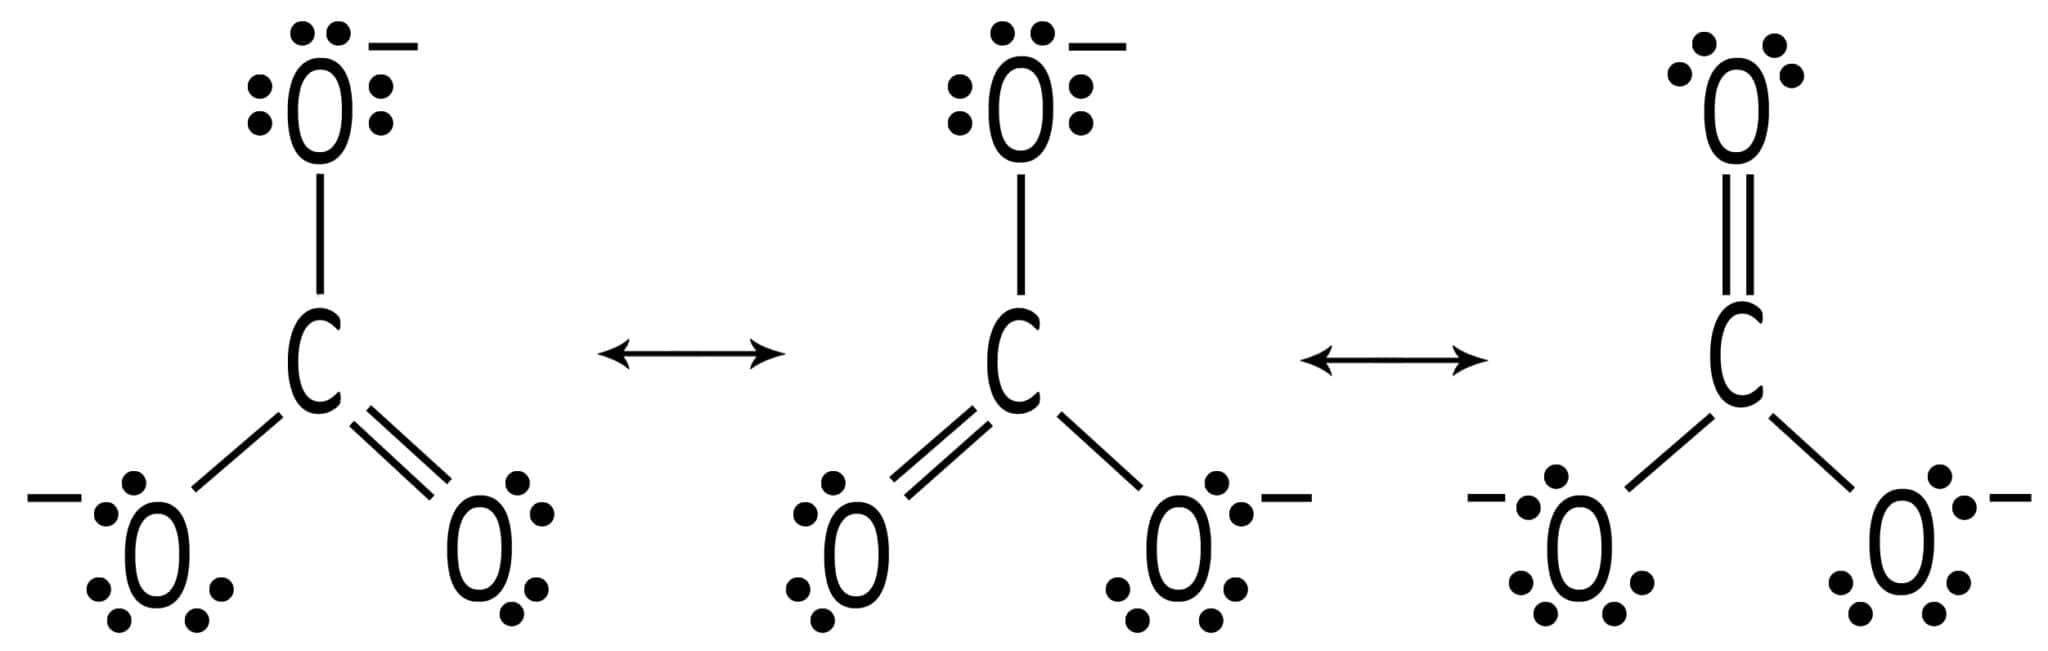
\includegraphics[width=0.75\linewidth]{Immagini/ione_carbonato_risonanza.jpg}
    \caption{Risonanza dello ione carbonato}
\end{figure}

\newpage
\section{Teoria VSEPR}
La \textbf{geometria molecolare} è la disposizione nel piano o nello spazio degli atomi di una molecola. 
La disposizione è determinata dal legame covalente che per formarsi necessita di una particolare disposizione.
Per determinare la formula di struttura dobbiamo usare la \textbf{teoria VSEPR Valence Shell Electron Pair Repulsion}.
Questa teoria si basa sul modello della repulsione degli elettroni che si trovano sullo strato di valenza. 
Per determinare la geometria usiamo la formula 
\begin{center}
    \textbf{ $AX_nE_m$}
\end{center}
Dove A indica l'atomo che si trova al centro della formula di struttura.
$X_n$ indica l'atomo centrale e n il numero di legami che forma
$E_m$ indica i doppietti di non legame (gli elettroni che non sono legati sempre e solo sull'atomo centrale).
Per determinare la struttura di usa il \textbf{Numero sterico} NS, che si trova come 
\begin{center}
    $NS = X_n + E_m$
\end{center}
Da quel risultato otteniamo che se NS vale: 
\begin{itemize}
    \item 2: \textbf{Lineare};
    \item 3: \textbf{Trigonale planare}, se non ci sono elettroni liberi;
    \item 3: \textbf{Angolata}, due legami e un non legame;
    \item 4: \textbf{Tetraedrica} 4 legami;
    \item 4: \textbf{Piramidale trigonale} tre legami e un non legame;
    \item 4: \textbf{Angolata} due legami e due non legami;
    \item 5: \textbf{Bipiramidale trigonale} solo legami;
    \item 6: \textbf{Ottaedrica} solo legami;
    \item 7: \textbf{Bipiramidale pentagonale};
\end{itemize}
L'\textbf{ibridazione} si può determinare sempre con il numero sterico ragionando in questo modo.
Se NS vale 3 significa che sono coinvolti tre orbitali dunque s(ha solo uno spazio) + 2 p (orbitale dopo s) nonchè $sp^2$.
\newpage
\section{Teoria OM e VB }
La teoria VB riesce a descrivere correttamente la geometria di moltissime molecole ma non permette di prevedere alcune proprietà fisiche quali gli spettri elettronici e le proprietà magnetiche.
Nella teoria VB, una molecola è visualizzata come un gruppo di atomi legati tra loro mediante la sovrapposizione localizzata di orbitali atomici del livello di
valenza. Nella teoria degli orbitali molecolari (MO) una molecola è visualizzata come un insieme di nuclei aventi orbitali elettronici delocalizzati sull'intera molecola.
La \textbf{teoria degli orbitali molecolari} è basata
sull'uso di orbitali molecolari, cioè di orbitali che si
estendono attorno ai nuclei dell'intera molecola: gli orbitali
molecolari sono funzioni d'onda che descrivono la
probabilità di trovare l'elettrone nello spazio attorno ai
nuclei della molecola. Come un atomo ha orbitali atomici che hanno una data energia e una data forma e sono occupati da elettroni, così una molecola ha orbitali molecolari che hanno una data energia ed una data forma e sono occupati dagli elettroni della molecola.
Il numero totale di orbitali molecolari OM che si formano è sempre uguale al numero di orbitali atomici che si sono combinati. Esistono due tipi di legame:
\begin{itemize}
    \item  \textbf{I leganti} hanno la maggior parte della densità elettronica tra i nuclei ed hanno energia inferiore a quella degli orbitali atomici.
    \item Negli \textbf{antileganti}, la maggior parte della densità elettronica non si trova tra i nuclei e sono quindi ad energia maggiore.
\end{itemize}
Per valutare se una molecola esista o meno bisogna studiare l'ordine di legame (O...L) definito come:
\begin{center}
    $\frac{\text{n°elettroni in orbitali leganti}- \text{n°elettroni in orbitali antileganti}}{2}$
\end{center}
Per \ce{H_2} si ha ordine di legame = $\frac{2-0}{2}$ = 1 esiste.
Per \ce{H_2^+} si ha ordine di legame = $\frac{1-0}{2}$ = $\frac{1}{2}$ 
esiste.
Per \ce{He_2} si ha ordine di legame = $\frac{2-2}{2}$ = 0 non esiste.
Per \ce{He_2^+ }si ha ordine di legame = $\frac{2-1}{2}$= $\frac{1}{2}$ così, può esistere.
\\
Dunque riassumendo le regole: 
\begin{enumerate}
    \item Da n orbitali atomici si ottengono, per combinazione lineare, n orbitali molecolari (MO);
    \item Gli MO leganti hanno energia minore degli MO antileganti;
    \item Gli elettroni si dispongono via via su orbitali ad energia crescente;
    \item Gli orbitali atomici si combinano tra loro in modo più efficace se hanno energie simili;
\end{enumerate}
Ricordare inoltre che: Per le molecole biatomiche del secondo periodo dobbiamo considerare anche gli orbitali molecolari derivanti dalle combinazioni lineari degli orbitali atomici 2s e 2p.

\newpage


\section{Orbitali molecolari delle molecole biatomiche}

La sezione sulla teoria OM introdotta nel capitolo sui composti si ferma a \ce{H2} e
\ce{He2}, dove esistono solo orbitali $\sigma$. Negli scritti, però, la richiesta è quasi
sempre relativa a molecole del secondo periodo --- \ce{O2}, \ce{N2}, \ce{NO}, \ce{CN-} ---
e chiede tre cose insieme: il diagramma energetico, l'ordine di legame e il carattere
para\-/diamagnetico. Questo capitolo fornisce lo schema da memorizzare e la procedura per
applicarlo in pochi minuti.

\subsection{Dagli orbitali atomici a quelli molecolari}

Combinando linearmente due orbitali atomici si ottengono sempre due orbitali molecolari:
uno \textbf{legante}, a energia inferiore (combinazione in fase, densità elettronica
concentrata fra i nuclei) e uno \textbf{antilegante}, a energia superiore e contrassegnato
dall'asterisco (combinazione fuori fase, con un piano nodale fra i nuclei).

La simmetria della sovrapposizione determina il tipo di orbitale:

\begin{itemize}
  \item i due orbitali $2s$ danno $\sigma_{2s}$ e $\sigma^*_{2s}$;
  \item i due orbitali $2p_z$, diretti lungo l'asse di legame, si sovrappongono frontalmente
        e danno $\sigma_{2p}$ e $\sigma^*_{2p}$;
  \item i quattro orbitali $2p_x$ e $2p_y$, perpendicolari all'asse, si sovrappongono
        lateralmente e danno due $\pi_{2p}$ \textbf{degeneri} e due $\pi^*_{2p}$
        \textbf{degeneri}.
\end{itemize}

Il numero totale di orbitali molecolari è sempre uguale al numero di orbitali atomici di
partenza. Il riempimento segue le stesse regole della configurazione elettronica atomica:
energia crescente (Aufbau), massimo due elettroni per orbitale (Pauli), e negli orbitali
degeneri gli elettroni si dispongono prima singolarmente con spin paralleli (Hund).

\subsection{I due ordinamenti energetici del secondo periodo}

Questo è il punto che va imparato a memoria, perché non è deducibile e decide tutto il
resto. L'ordine relativo di $\sigma_{2p}$ e $\pi_{2p}$ cambia a metà periodo:

\begin{center}
\begin{tabular}{ll}
  \toprule
  Molecole & Ordinamento (energia crescente) \\
  \midrule
  \ce{Li2}, \ce{Be2}, \ce{B2}, \ce{C2}, \ce{N2}
    & $\sigma_{2s} < \sigma^*_{2s} < \pi_{2p} < \sigma_{2p} < \pi^*_{2p} < \sigma^*_{2p}$ \\[2pt]
  \ce{O2}, \ce{F2}, \ce{Ne2}
    & $\sigma_{2s} < \sigma^*_{2s} < \sigma_{2p} < \pi_{2p} < \pi^*_{2p} < \sigma^*_{2p}$ \\
  \bottomrule
\end{tabular}
\end{center}

\noindent La ragione è il \textbf{mescolamento $s$--$p$}: negli elementi a sinistra del
periodo gli orbitali $2s$ e $2p$ hanno energie relativamente vicine e interagiscono,
innalzando $\sigma_{2p}$ sopra $\pi_{2p}$. In ossigeno e fluoro la carica nucleare efficace
è maggiore, il $2s$ scende molto in energia, il mescolamento diventa trascurabile e
l'ordine ``naturale'' viene ripristinato.

\medskip
\noindent\emph{Regola pratica:} fino all'azoto (\ce{Z} $\leq 7$) i $\pi$ stanno
\textbf{sotto}; da ossigeno in poi ($Z \geq 8$) i $\pi$ stanno \textbf{sopra} il
$\sigma_{2p}$.

\subsection{Ordine di legame}

L'ordine di legame quantifica quanti legami netti tengono insieme la molecola:

\begin{equation}
  \text{O.L.} = \frac{n_{\text{leganti}} - n_{\text{antileganti}}}{2}
\end{equation}

Le conseguenze fisiche sono immediate e vengono chieste sistematicamente:

\begin{itemize}
  \item O.L. maggiore $\Rightarrow$ legame più \textbf{forte} (maggiore energia di legame);
  \item O.L. maggiore $\Rightarrow$ legame più \textbf{corto} (minore distanza internucleare);
  \item O.L. $= 0$ $\Rightarrow$ la molecola \textbf{non esiste} come specie stabile.
\end{itemize}

\noindent Ordinare tre specie per distanza di legame crescente significa quindi ordinarle
per ordine di legame \emph{decrescente}.

\subsection{Proprietà magnetiche}

\begin{itemize}
  \item \textbf{Paramagnetica}: possiede almeno un elettrone spaiato; è attratta da un
        campo magnetico;
  \item \textbf{Diamagnetica}: tutti gli elettroni sono appaiati; è debolmente respinta.
\end{itemize}

Il caso storicamente decisivo è \ce{O2}: la teoria di Lewis, che ne prevede il doppio
legame con tutti gli elettroni appaiati, non spiega il paramagnetismo sperimentale
dell'ossigeno, mentre la teoria OM lo predice correttamente. È l'argomento da citare quando
il compito chiede ``perché la teoria OM è superiore alla VB''.

\subsection{Procedura operativa}

\begin{enumerate}
  \item Contare gli \textbf{elettroni di valenza} totali, aggiungendo un elettrone per ogni
        carica negativa e sottraendone uno per ogni carica positiva.
  \item Scegliere l'ordinamento in base agli atomi coinvolti (regola dell'azoto).
  \item Riempire gli orbitali in ordine di energia crescente applicando Hund.
  \item Contare elettroni leganti e antileganti e calcolare l'ordine di legame.
  \item Verificare la presenza di elettroni spaiati per il carattere magnetico.
\end{enumerate}

\subsubsection{Esempio guidato: la serie dell'ossigeno}

\emph{Scrivere il diagramma degli orbitali molecolari di \ce{O2}, \ce{O2+} e \ce{O2^-},
determinare l'ordine di legame, dire se sono para- o diamagnetiche e ordinarle per distanza
di legame crescente.}

\medskip
\noindent Tutte e tre usano l'ordinamento con $\sigma_{2p}$ sotto i $\pi_{2p}$.

\medskip
\noindent\textbf{\ce{O2}} --- $6 + 6 = 12$ elettroni di valenza:
\begin{equation*}
  \sigma_{2s}^2 \, \sigma_{2s}^{*2} \, \sigma_{2p}^2 \, \pi_{2p}^4 \, \pi_{2p}^{*2}
\end{equation*}
I due elettroni nei $\pi^*$ occupano orbitali degeneri e per Hund restano \textbf{spaiati}.
Leganti $= 8$, antileganti $= 4$, quindi $\text{O.L.} = (8-4)/2 = 2$.
Molecola \textbf{paramagnetica}.

\medskip
\noindent\textbf{\ce{O2+}} --- $11$ elettroni: si toglie un elettrone da $\pi^*$, che resta
con uno solo. Leganti $=8$, antileganti $=3$, $\text{O.L.} = 2{,}5$. Un elettrone spaiato:
\textbf{paramagnetica}.

\medskip
\noindent\textbf{\ce{O2^-}} --- $13$ elettroni: i $\pi^*$ ospitano tre elettroni.
Leganti $=8$, antileganti $=5$, $\text{O.L.} = 1{,}5$. Un elettrone spaiato:
\textbf{paramagnetica}.

\medskip
\noindent\textbf{Ordinamento.} Poiché la distanza cresce al diminuire dell'ordine di legame:
\begin{equation*}
  \ce{O2+} \; (2{,}5) \;<\; \ce{O2} \; (2) \;<\; \ce{O2^-} \; (1{,}5)
\end{equation*}
Rimuovere un elettrone da \ce{O2} \emph{rafforza} il legame, perché l'elettrone tolto era
antilegante: è un risultato controintuitivo che vale la pena saper motivare.

\subsubsection{Esempio guidato: specie isoelettroniche}

\emph{Determinare ordine di legame e proprietà magnetiche di \ce{NO}, \ce{NO+} e \ce{CN-}.}

\medskip
Per le biatomiche eteronucleari di atomi vicini nella tavola periodica si usa lo stesso
schema delle omonucleari, con lo scheletro dell'azoto ($\pi$ sotto $\sigma_{2p}$). Il
risultato per l'ordine di legame non dipende comunque da questa scelta, perché il conteggio
di leganti e antileganti resta lo stesso.

\begin{center}
\begin{tabular}{lccl}
  \toprule
  Specie & $e^-$ di valenza & O.L. & Carattere magnetico \\
  \midrule
  \ce{NO}  & $5+6 = 11$    & $2{,}5$ & paramagnetica (1 $e^-$ in $\pi^*$) \\
  \ce{NO+} & $10$          & $3$     & diamagnetica \\
  \ce{NO^-}& $12$          & $2$     & paramagnetica (2 $e^-$ spaiati) \\
  \ce{CN-} & $4+5+1 = 10$  & $3$     & diamagnetica \\
  \ce{N2}  & $10$          & $3$     & diamagnetica \\
  \bottomrule
\end{tabular}
\end{center}

\noindent \ce{CN-}, \ce{NO+}, \ce{N2} e \ce{CO} hanno tutte $10$ elettroni di valenza: sono
\textbf{isoelettroniche} e condividono ordine di legame $3$ e carattere diamagnetico. Se
riconosci l'isoelettronicità con \ce{N2}, l'esercizio è risolto senza scrivere il diagramma.

\subsubsection{Esempio guidato: una biatomica molto asimmetrica}

\emph{Scrivere il diagramma degli orbitali molecolari e la configurazione elettronica di
\ce{HCl}, indicando ordine di legame ed eventuale paramagnetismo.}

\medskip
Qui i due atomi hanno energie orbitaliche molto diverse, quindi lo schema del secondo
periodo non si applica. Si combina efficacemente solo l'orbitale $1s$ dell'idrogeno con il
$3p_z$ del cloro (quello diretto lungo l'asse di legame), generando $\sigma$ e $\sigma^*$.
Gli orbitali $3s$, $3p_x$ e $3p_y$ del cloro non trovano partner di simmetria ed energia
adeguate: restano \textbf{non leganti} e ospitano i doppietti solitari.

Con $1 + 7 = 8$ elettroni di valenza la configurazione è
\begin{equation*}
  \sigma^2 \; (3s)^2 \; (3p_x)^2 \; (3p_y)^2
\end{equation*}
Gli orbitali non leganti non entrano nel conteggio, quindi
$\text{O.L.} = (2-0)/2 = 1$. Nessun elettrone spaiato: molecola \textbf{diamagnetica}.
Poiché il $\sigma$ legante somiglia più al $3p_z$ del cloro che all'$1s$ dell'idrogeno, la
densità elettronica è spostata verso il cloro: è la descrizione in linguaggio OM della
polarità del legame.

\subsection{Esercizi di verifica}

\begin{enumerate}
  \item Costruire il diagramma di \ce{N2} e di \ce{N2+} e spiegare perché la ionizzazione
        dell'azoto \emph{indebolisce} il legame, contrariamente a quanto accade
        per \ce{O2}.
  \item \ce{B2} è paramagnetica e \ce{C2} diamagnetica. Verificare che entrambi i risultati
        seguono dall'ordinamento con $\pi_{2p}$ sotto $\sigma_{2p}$, e mostrare che
        l'ordinamento opposto darebbe previsioni sbagliate.
  \item Ordinare \ce{F2}, \ce{F2+} e \ce{F2^-} per energia di legame decrescente.
  \item Perché \ce{He2} non esiste mentre \ce{He2+} può esistere?
\end{enumerate}

\section{Formule e composizione percentuale}
Attraverso le formule chimiche si può risalire alla percentuale di massa o composizione percentuale di ciascun elemento nel composto. 
La \textbf{composizione percentuale} può aiutare nel determinare la massa effettiva di un elemento nel composto.
La \textbf{formula minima} indica il rapporto di combinazione minimo con cui gli atomi si legano per formare i prodotti. Esistono pochi passaggi per determinarla:
\begin{enumerate}
    \item scrivere la massa m in grammi di ciascun elemento presente in 100 g di composto, cioè la sua percentuale in massa;
    \item si calcola il numero di moli di ciascun elemento;
    \item si divide il numero di moli di ciascun elemento per il più piccolo numero di moli calcolate, ii numeri ottenuti sono gli indici numerici della formula;
    \item si scrivono gli elementi con l'indice ricavato;
\end{enumerate}
E' possibile determina anche la \textbf{formula molecolare}, dovremmo calcolare il peso molecolare a partire dalla formula minima dividere il peso sperimentale con quello teorico, otteniamo il fattore di
\textbf{moltiplicazione}, moltiplichiamo tutto per ottenere la formula.
Per determinare la composizione percentuale si può fare:
\begin{center}
   \textbf{ $ \% = \frac{grammi dell'elemento}{g della massa totale} \cdot 100$}
\end{center}
\section{Esempio guidati sul ricavo delle formule}
Cerchiamo di determinare la \textbf{formula minima} di un composto formato da \ce{Hg e O}, conoscendone la grammatura rispettivamente $43.6 e 3.7$.
\begin{itemize}
    \item troviamo la massa totale del composto: PM = $43.6 + 3.7 = 50 \text{g}$;
    \item Con la tavola individuo i pesi atomici degli elementi;
    \item Trovo la mole di ciascun elemento (con la formula di prima); $n_{Hg}= 0.23 \text{mol};
 \\ n_O= 0.23 \text{mol}$
    \item Dividendo tutto per 0.23 (per intenderci meglio qui non c'è un numero più basso quindi è semplicemente 0.23 : 0.23 che fa 1)ottengo 1 dunque il rapporto è 1 : 1;
    \item La formula minima è \ce{HgO} (\textit{se metti caso fosse stato 2:1 avrei dovuto scrivere \ce{Hg_2O}})
\end{itemize}
Si potrebbe fare anche conoscendo la composizione percentuale  poichè  indica quanti grammi dell'elemento sono presenti in 100 g di
composto; dunque una volta trovati i grammi di ciascun elemento in realtà già forniti ripeto i passaggi.
Individuiamo ora la \textbf{formula molecolare} sapendo che il PM= 180 g/mol (quello sperimentale). Abbiamo la formula minima \ce{CH_2O}.
\begin{itemize}
    \item Sappiamo che il $\text{PM}_{\ce{CH_2}} = 30 \text{ g/mol}$;
    \item Dividiamo il peso sperimentale con quello teorico
    \begin{center}
        $\frac{180 g/mol}{30 g/mol} = 6$ 
    \end{center} 
    \item La formula sarà dunque \ce{C_6H_12O_6}, quel 12 all'idrogeno deriva dal 2 della formula minima per 6 trovato;
\end{itemize}
Ultimo esempio è sulla \textbf{determinazione della formula percentuale}. Per determinarla seguiamo questi passaggi:
\begin{itemize}
    \item Conosciamo la massa degli elementi;
    \item Troviamo la massa totale;
    \item Dividiamo massa di ogni elementi su quella totale e moltiplichiamo per 100;
    \item Troveremo la composizone percentule di ciascun elemento;
\end{itemize}
Se siamo a conoscenza della formula minima allora risaliamo ai pesi molecolari di ciascun elemento e quello totale, poi ripetiamo il calcolo di prima.
\newpage

La \textbf{resa di una reazione} dice quanto prodotto si forma solo raramente può dirsi quantitativa,
normalmente la quantità di prodotto ottenibile in una data
reazione è sempre inferiore al valore teorico deducibile dalla
stechiometria, ad esempio per la formazione di coprodotti di
reazione. 
Si definisce resa di una reazione chimica
il rapporto tra le moli di prodotto ottenuto
rispetto alle moli del prodotto calcolato dai reagenti. 
Un \textbf{elettrolita}  una sostanza che si scioglie in acqua
producendo ioni (dissociazione) e formando una soluzione che
conduce l'elettricità. Si classificano in:
\begin{itemize}
    \item \textbf{Forti}, ha una dissociazione ionica completa;
    \item \textbf{Deboli}, ha una dissociazioni ionica parziale meglio dire non completa;
\end{itemize}
Prima di affrontare le reazioni Redox (nonchè quelle di ossidazione e riduzione) è necessario introdurre il concetto di \textbf{ione spettatore} ,sono ioni presenti in una soluzione che non partecipano direttamente a una reazione chimica
\

\newpage

\section{Acidi, basi e reazioni redox}
Esistono diverse definizioni attribuite ad acido e base, tre in particolare:
\begin{itemize}
    \item \textbf{Brønsted--Lowry}: acido è ciò che cede \ce{H+}, base è ciò che acquista \ce{H+}. A differenza della definizione di Arrhenius, non è limitata alle soluzioni acquose. Da questa definizione deriva la coppia \textbf{acido--base coniugata}, i cui due membri differiscono per un solo ione \ce{H+};
    \item \textbf{Arrhenius}: acido è ciò che, disciolto in acqua, libera ioni \ce{H+}, mentre base è ciò che in acqua libera ioni \ce{OH-}. Il limite di questa definizione è che funziona solo nelle soluzioni acquose;
    \item \textbf{Lewis}: acido è la specie che accetta un doppietto elettronico, base è la specie che cede un doppietto elettronico. Questa è la definizione più ampia e completa.
\end{itemize}
Con il termine \textbf{reazione redox} si intendono tutte quelle reazioni che avvengono con trasferimento di elettroni. Si distinguono due reagenti:
\begin{itemize}
    \item \textbf{Riducente}: la specie che \textbf{cede} elettroni e quindi \textbf{aumenta} il suo numero di ossidazione (si ossida). In genere si tratta di un metallo, che ha bassa energia di ionizzazione;
    \item \textbf{Ossidante}: la specie che \textbf{acquista} elettroni e quindi \textbf{diminuisce} il suo numero di ossidazione (si riduce).
\end{itemize}
Il \textbf{numero di ossidazione} indica la carica che quell'atomo avrebbe se nel composto tutti i legami fossero di tipo ionico. Ci sono sei regole generali da tenere a mente:
\begin{enumerate}
    \item In un composto neutro la sommatoria dei numeri di ossidazione è nulla; in uno ione poliatomico è pari alla carica dello ione;
    \item Nelle sostanze elementari il numero di ossidazione è zero;
    \item I metalli alcalini hanno numero di ossidazione $+1$. L'idrogeno ha quasi sempre $+1$, tranne negli idruri metallici dove assume $-1$;
    \item I metalli alcalino terrosi hanno numero di ossidazione $+2$;
    \item L'ossigeno ha generalmente $\mathbf{-2}$, tranne nei perossidi dove assume $-1$.
    \item Gli alogeni hanno numero di ossidazione $-1$ nella maggior parte dei composti; possono assumere valori positivi solo se legati a elementi più elettronegativi (ossigeno o un alogeno più leggero). Il fluoro fa eccezione: è sempre $-1$.
\end{enumerate}
\newpage
\section{Bilanciamento Redox}
Quando una reazione avviene in \ce{H2O} e non è bilanciata, il metodo da seguire è quello delle \textbf{semireazioni}. Tale metodo si applica seguendo queste regole:

\begin{enumerate}
    \item \textbf{Riconoscere l'ambiente di reazione.} Prima di iniziare bisogna sapere in che ambiente si lavora, perché questo determina quali specie è lecito aggiungere:
    \begin{itemize}
        \item \textbf{ambiente acido}: compaiono \ce{H2SO4}, \ce{HCl}, \ce{HNO3}, \ce{H+}. Si possono aggiungere \ce{H+} e \ce{H2O};
        \item \textbf{ambiente basico}: compaiono \ce{NaOH}, \ce{KOH}, \ce{OH-}. Si possono aggiungere \ce{OH-} e \ce{H2O}.
    \end{itemize}
    \textit{In ambiente acido non si può mai scrivere \ce{OH-}, e in ambiente basico non si può mai scrivere \ce{H+}: sarebbero specie che in quelle condizioni non esistono in concentrazione apprezzabile.}

    \item \textbf{Assegnare i numeri di ossidazione.} Si calcolano i n.o. di tutti gli atomi in reagenti e prodotti e si individuano i due elementi che li cambiano:
    \begin{itemize}
        \item l'elemento che \textbf{aumenta} il n.o. \textbf{si ossida}, e la sua specie è il \textbf{riducente};
        \item l'elemento che \textbf{diminuisce} il n.o. \textbf{si riduce}, e la sua specie è l'\textbf{ossidante}.
    \end{itemize}

    \item \textbf{Scrivere le due semireazioni in forma ionica.} Si separa la reazione in due semireazioni, ciascuna contenente solo la specie che contiene l'elemento che cambia n.o., con la sua carica corretta. Gli ioni spettatori si lasciano fuori. Se la reazione è data in forma molecolare, si dissociano prima gli elettroliti forti.

    \item \textbf{Bilanciare l'elemento che cambia numero di ossidazione.} Si mettono i coefficienti necessari perché l'atomo protagonista risulti bilanciato nei due membri della semireazione (ad esempio \ce{2S2O3^2- -> S4O6^2-}, non \ce{S2O3^2- -> S4O6^2-}).

    \item \textbf{Bilanciare ossigeno e idrogeno.} È l'unico passaggio in cui i due ambienti si comportano diversamente.
    \begin{itemize}
        \item \textbf{In ambiente acido}: si aggiunge \ce{H2O} dal lato che ha meno ossigeni, tante quante ne mancano, e poi \ce{H+} dall'altro lato per bilanciare gli idrogeni introdotti.
        \item \textbf{In ambiente basico} (metodo in due tempi, il più sicuro): si bilancia come se si fosse in ambiente acido, con \ce{H2O} e \ce{H+}; poi si aggiungono a \textbf{entrambi} i membri tanti \ce{OH-} quanti sono gli \ce{H+} presenti; dal lato in cui si incontrano avviene \ce{H+ + OH^- -> H2O}; infine si semplificano le molecole d'acqua presenti da entrambe le parti.
        \item \textit{Metodo diretto per l'ambiente basico}: per ogni ossigeno mancante da un lato si aggiungono \ce{2OH^-} su quel lato e \ce{1H2O} sull'altro. È più veloce, ma si sbaglia più facilmente il verso.
    \end{itemize}

    \item \textbf{Bilanciare le cariche con gli elettroni.} Si somma algebricamente la carica di ciascun membro e si aggiungono gli elettroni dove serve per pareggiarla:
    \begin{itemize}
        \item semireazione di \textbf{ossidazione}: elettroni \textbf{a destra}, tra i prodotti;
        \item semireazione di \textbf{riduzione}: elettroni \textbf{a sinistra}, tra i reagenti.
    \end{itemize}
    Come verifica, il numero di elettroni deve coincidere con la variazione di n.o. calcolata al punto 2, moltiplicata per il numero di atomi coinvolti; se non torna, c'è un errore nei passaggi precedenti.

    \item \textbf{Pareggiare gli elettroni.} Si moltiplica ciascuna semireazione per un fattore tale che gli elettroni ceduti siano uguali a quelli acquistati (minimo comune multiplo).

    \item \textbf{Sommare e semplificare.} Si sommano le due semireazioni membro a membro e si semplificano gli elettroni (che spariscono sempre del tutto), le \ce{H2O} e gli \ce{H+} (o \ce{OH-}) presenti da entrambi i lati.

    \item \textbf{Verificare.} Due controlli, entrambi obbligatori:
    \begin{itemize}
        \item \textbf{bilancio di massa}: ogni elemento deve avere lo stesso numero di atomi nei due membri;
        \item \textbf{bilancio di carica}: la somma algebrica delle cariche deve essere uguale nei due membri (non necessariamente nulla).
    \end{itemize}

    \item \textbf{Tornare alla forma molecolare}, se richiesto: si reintroducono gli ioni spettatori, in numero uguale da entrambi i lati, ricostruendo i composti di partenza.
\end{enumerate}

\subsection{Esempio in ambiente acido}
\begin{center}
    \ce{MnO4^- + Fe^2+ -> Mn^2+ + Fe^3+}
\end{center}
Il manganese passa da $+7$ a $+2$: si riduce acquistando 5 elettroni. Il ferro passa da $+2$ a $+3$: si ossida cedendo 1 elettrone.

\textbf{Semireazione di riduzione.} Mancano 4 ossigeni a destra, quindi aggiungo \ce{4H2O} a destra e \ce{8H+} a sinistra. Le cariche sono $-1+8 = +7$ a sinistra e $+2$ a destra, quindi servono 5 elettroni a sinistra:
\[
\ce{MnO4^- + 8H^+ + 5e^- -> Mn^2+ + 4H2O}
\]

\textbf{Semireazione di ossidazione}, da moltiplicare per 5:
\[
\ce{Fe^2+ -> Fe^3+ + e^-}
\]

\textbf{Somma finale:}
\[
\mathbf{\ce{MnO4^- + 8H^+ + 5Fe^2+ -> Mn^2+ + 4H2O + 5Fe^3+}}
\]
Verifica delle cariche: a sinistra $-1 + 8 + 10 = +17$, a destra $+2 + 15 = +17$.

\subsection{Esempio in ambiente basico}
\begin{center}
    \ce{MnO4^- + SO3^2- -> MnO2 + SO4^2-}
\end{center}
Il manganese passa da $+7$ a $+4$ (3 elettroni), lo zolfo da $+4$ a $+6$ (2 elettroni).

\textbf{Semireazione di riduzione.} Mancano 2 ossigeni a destra: con il metodo diretto aggiungo \ce{4OH^-} a destra e \ce{2H2O} a sinistra. Le cariche sono $-1$ a sinistra e $-4$ a destra, quindi servono 3 elettroni a sinistra:
\[
\ce{MnO4^- + 2H2O + 3e^- -> MnO2 + 4OH^-}
\]

\textbf{Semireazione di ossidazione.} Manca 1 ossigeno a sinistra: aggiungo \ce{2OH^-} a sinistra e \ce{H2O} a destra. Le cariche sono $-4$ a sinistra e $-2$ a destra, quindi servono 2 elettroni a destra:
\[
\ce{SO3^2- + 2OH^- -> SO4^2- + H2O + 2e^-}
\]

\textbf{Pareggio degli elettroni:} riduzione $\times 2$, ossidazione $\times 3$ (m.c.m. $= 6$). Sommando e semplificando 3 \ce{H2O} e 6 \ce{OH-}:
\[
\mathbf{\ce{2MnO4^- + 3SO3^2- + H2O -> 2MnO2 + 3SO4^2- + 2OH^-}}
\]
Verifica delle cariche: a sinistra $-2 - 6 = -8$, a destra $-6 - 2 = -8$.

\medskip
\textit{Unica accortezza da tenere a mente: quando partiamo da una reazione in forma molecolare e la rendiamo ionica, alla fine ci troveremo con degli ioni; dobbiamo quindi ricombinare il tutto con i rispettivi ioni spettatori per tornare alla forma molecolare!}



\subsection{Reazioni redox di disproporzione}
Esistono reazioni in cui la stessa specie chimica si ossida e si riduce: tali reazioni vengono dette \textbf{reazioni di disproporzione} e si svolgono nello stesso modo delle normali reazioni redox.



\subsubsection*{Esempio: disproporzione in ambiente acido}
\begin{center}
    \ce{S2O3^2- + ClO^- -> S4O6^2- + Cl^-}
\end{center}
Lo zolfo si comporta contemporaneamente da riducente e da ossidante. Bilancio prima le masse dello zolfo:
\[
\ce{2S2O3^2- -> S4O6^2-}
\]
Ossigeni e idrogeni sono già bilanciati; bilancio le cariche con gli elettroni, ottenendo le due semireazioni:
\[
\ce{2S2O3^2- -> S4O6^2- + 2e^-}
\qquad\qquad
\ce{ClO^- + 2H^+ + 2e^- -> Cl^- + H2O}
\]
Gli elettroni sono già pareggiati (2 e 2): sommando e semplificando si ottiene la reazione bilanciata:
\[
\mathbf{\ce{2S2O3^2- + ClO^- + 2H^+ -> S4O6^2- + Cl^- + H2O}}
\]


\newpage

\section{Calcoli stechiometrici per le reazioni}
In una reazione chimica bilanciata i coefficienti stechiometrici indicano i rapporti molari tra le specie reagenti e quelle prodotte. Se si vuole studiare quantitativamente la massa necessaria alla reazione e quella prodotta si usa la seguente formula:
\begin{equation}
    n \; (mol) = \frac{m \; (g)}{MM \; (g/mol)}
\end{equation}
In generale, per analizzare quantitativamente una reazione bisogna scrivere 2 righe di una tabella sotto ogni reagente e prodotto, riportando il numero di moli nello stato iniziale e nello stato finale, come segue:

\begin{center}
\begin{tabular}{l c c c c c}
                    & \ce{P4_{(s)}} & $+$ & \ce{6Cl2_{(g)}} & $\longrightarrow$ & \ce{4PCl3_{(l)}} \\
\hline
Moli iniziali       & 0.01170 &  & 0.07020 &  & 0    \\
Moli finali         & 0 &  & 0 &  & 0.04680 \\
\end{tabular}
\end{center}

\subsection{Reagente limitante}
Se i reagenti non sono in un rapporto molare corretto, allora vi sarà un reagente limitante e 1 o più reagenti in eccesso.

Il reagente limitante si trova confrontando il rapporto stechiometrico dei reagenti (A e B) con il rapporto molare dei reagenti (A e B), dove:
\begin{itemize}
    \item il \textbf{rapporto stechiometrico} $\dfrac{\text{coeff}_A}{\text{coeff}_B}$ è quello \emph{richiesto} dalla reazione bilanciata;
    \item il \textbf{rapporto molare} $\dfrac{n_A}{n_B}$ è quello effettivamente \emph{disponibile}, calcolato dalle moli dei due reagenti.
\end{itemize}

\noindent
Confrontando i due rapporti, se:
\begin{itemize}
    \item $\dfrac{\text{coeff}_A}{\text{coeff}_B} < \dfrac{n_A}{n_B}$, allora ne serve relativamente poco di A rispetto a quanto ne è disponibile: il reagente limitante è \textbf{B}, mentre A è in eccesso;
    \item $\dfrac{\text{coeff}_A}{\text{coeff}_B} > \dfrac{n_A}{n_B}$, allora ne servirebbe più A di quanto ne è disponibile: il reagente limitante è \textbf{A}, mentre B è in eccesso;
    \item $\dfrac{\text{coeff}_A}{\text{coeff}_B} = \dfrac{n_A}{n_B}$, allora i due reagenti sono in rapporto stechiometrico esatto e si consumano completamente entrambi: non vi è né reagente limitante né eccesso.
\end{itemize}

\noindent
\textit{Il criterio si applica a coppie di reagenti: con tre o più reagenti conviene ripetere il confronto a due a due, oppure usare il metodo del quoziente $n/\text{coeff}$, in cui il valore più piccolo individua direttamente il limitante.}

\medskip
\noindent
Una volta individuato il reagente limitante, \textbf{tutti i calcoli sulle quantità di prodotto e sulla resa devono partire da esso}, mai dal reagente in eccesso.

\subsubsection{Esempio}
\begin{center}
    \ce{P4_{(s)} + 6Cl2_{(g)} -> 4PCl3_{(l)}}
\end{center}
Disponiamo di 62,0 g di \ce{P4} ($MM = 123{,}9$ g/mol) e di 200,0 g di \ce{Cl2} ($MM = 70{,}90$ g/mol):
\[
n_{\ce{P4}} = \frac{62{,}0}{123{,}9} = 0{,}500\ \mathrm{mol}
\qquad\qquad
n_{\ce{Cl2}} = \frac{200{,}0}{70{,}90} = 2{,}82\ \mathrm{mol}
\]
Confrontiamo i due rapporti, ponendo A $=$ \ce{P4} e B $=$ \ce{Cl2}:
\[
\frac{\text{coeff}_{\ce{P4}}}{\text{coeff}_{\ce{Cl2}}} = \frac{1}{6} = 0{,}167
\qquad\qquad
\frac{n_{\ce{P4}}}{n_{\ce{Cl2}}} = \frac{0{,}500}{2{,}82} = 0{,}177
\]
Poiché $0{,}167 < 0{,}177$, ci troviamo nel primo caso: il reagente limitante è il \textbf{cloro}, mentre il fosforo è in eccesso.

\medskip
\noindent
Da qui si ricavano le quantità in gioco, partendo sempre dal limitante:
\begin{itemize}
    \item prodotto teorico: $n_{\ce{PCl3}} = 2{,}82 \cdot \dfrac{4}{6} = 1{,}88$ mol;
    \item fosforo consumato: $n_{\ce{P4}} = 2{,}82 \cdot \dfrac{1}{6} = 0{,}470$ mol;
    \item fosforo residuo: $0{,}500 - 0{,}470 = 0{,}030$ mol.
\end{itemize}

% Capitolo da inserire in Appunti_Chimica.tex
% Richiede nel preambolo: \usepackage[version=4]{mhchem}, amsmath, booktabs
% Collocazione consigliata: dopo il Capitolo 2 (Composti e reazioni),
% prima del capitolo su soluzioni, cinetica ed equilibrio.

\chapter{Termochimica e termodinamica chimica}

Una reazione chimica non si limita a trasformare materia: scambia anche energia con
l'ambiente. Sapere \emph{quanta} energia viene liberata o assorbita, e sapere se una
reazione avverrà spontaneamente oppure no, sono due domande distinte a cui rispondono
due grandezze diverse: l'entalpia $\Delta H$ e l'energia libera $\Delta G$. Questo
capitolo serve a rispondere a entrambe.

\section{Sistema, ambiente e funzioni di stato}

Chiamiamo \textbf{sistema} la porzione di universo che stiamo studiando (i reagenti nel
recipiente) e \textbf{ambiente} tutto il resto. Il calore scambiato si indica con $Q$ e
si adotta la convenzione:

\begin{itemize}
  \item $Q < 0$: il sistema \emph{cede} calore all'ambiente, reazione \textbf{esotermica};
  \item $Q > 0$: il sistema \emph{assorbe} calore, reazione \textbf{endotermica}.
\end{itemize}

Una \textbf{funzione di stato} è una grandezza il cui valore dipende solo dallo stato
iniziale e finale del sistema, non dal percorso seguito per andare dall'uno all'altro.
L'entalpia $H$ è una funzione di stato; il calore $Q$ in generale non lo è, ma a
pressione costante (il caso di quasi tutte le reazioni di laboratorio) vale

\begin{equation}
  Q_p = \Delta H
\end{equation}

ed è per questo che l'entalpia è la grandezza termochimica di riferimento. Il fatto che
$H$ sia funzione di stato è ciò che rende possibile tutto il resto del capitolo: possiamo
calcolare il $\Delta H$ di una reazione sommando i $\Delta H$ di reazioni fittizie, purché
partano e arrivino agli stessi composti.


\section{Stato standard ed entalpia di formazione}

Lo \textbf{stato standard} di una sostanza è la sua forma più stabile alla pressione di
$1$ bar e alla temperatura specificata (convenzionalmente $298{,}15$~K, cioè $25\,^\circ$C).
Si indica con l'apice $^\circ$.

L'\textbf{entalpia standard di formazione} $\Delta H^\circ_f$ di un composto è la
variazione di entalpia associata alla formazione di \emph{una mole} di quel composto a
partire dagli elementi costituenti presi nel loro stato standard.

\begin{itemize}
  \item Per definizione, $\Delta H^\circ_f = 0$ per ogni \textbf{elemento} nella sua forma
        più stabile: \ce{O2(g)}, \ce{N2(g)}, \ce{H2(g)}, \ce{C} (grafite), \ce{Cl2(g)},
        \ce{Br2(l)}, \ce{Hg(l)}, i metalli solidi.
  \item Attenzione allo stato fisico: $\Delta H^\circ_f(\ce{H2O(l)}) = -286$~kJ/mol, ma
        $\Delta H^\circ_f(\ce{H2O(g)}) = -242$~kJ/mol. Negli esercizi l'acqua prodotta da
        una combustione è quasi sempre \emph{liquida}.
  \item Un $\Delta H^\circ_f$ molto negativo indica un composto stabile rispetto ai suoi
        elementi.
\end{itemize}

\section{La legge di Hess}

Poiché $H$ è una funzione di stato, il $\Delta H$ di una reazione è lo stesso sia che essa
avvenga in un solo stadio, sia che avvenga attraverso una serie di stadi intermedi.
Operativamente questo significa che le equazioni termochimiche si possono manipolare come
equazioni algebriche:

\begin{itemize}
  \item se si \textbf{inverte} una reazione, $\Delta H$ cambia di segno;
  \item se si \textbf{moltiplica} una reazione per un coefficiente $n$, anche $\Delta H$
        va moltiplicato per $n$;
  \item se si \textbf{sommano} due reazioni, i rispettivi $\Delta H$ si sommano.
\end{itemize}

La conseguenza più usata negli esercizi è la formula generale

\begin{equation}
  \Delta H^\circ_{\text{reaz}} = \sum_{\text{prodotti}} \nu_i \, \Delta H^\circ_{f,i}
                               - \sum_{\text{reagenti}} \nu_j \, \Delta H^\circ_{f,j}
  \label{eq:hess}
\end{equation}

dove $\nu$ sono i coefficienti stechiometrici della reazione \emph{bilanciata}.


\section{Lo schema d'esame: $\Delta H^\circ_f$ da $\Delta H^\circ_{\text{comb}}$}

Il compito ricorrente è sempre lo stesso: viene fornita l'entalpia di combustione di un
composto organico e le entalpie di formazione di \ce{CO2(g)} e \ce{H2O(l)}, e si chiede
l'entalpia di formazione del composto. Il metodo è applicare
\eqref{eq:hess} alla reazione di combustione e risolvere rispetto all'unica incognita.

\subsection{Esempio guidato: il propano}

\emph{Calcolare $\Delta H^\circ_f$ del propano \ce{C3H8(g)} sapendo che
$\Delta H^\circ_{\text{comb}} = -2221$~kJ/mol, con
$\Delta H^\circ_f(\ce{CO2(g)}) = -394$~kJ/mol e
$\Delta H^\circ_f(\ce{H2O(l)}) = -286$~kJ/mol.}

\medskip
\noindent\textbf{Passo 1 --- scrivere e bilanciare la combustione.}
\begin{equation*}
  \ce{C3H8(g) + 5 O2(g) -> 3 CO2(g) + 4 H2O(l)}
\end{equation*}

\noindent\textbf{Passo 2 --- applicare \eqref{eq:hess}}, ricordando che
$\Delta H^\circ_f(\ce{O2}) = 0$:
\begin{equation*}
  \Delta H^\circ_{\text{comb}}
  = \Big[ 3\,\Delta H^\circ_f(\ce{CO2}) + 4\,\Delta H^\circ_f(\ce{H2O}) \Big]
  - \Big[ \Delta H^\circ_f(\ce{C3H8}) \Big]
\end{equation*}

\noindent\textbf{Passo 3 --- sostituire e risolvere.}
\begin{align*}
  -2221 &= \big[ 3(-394) + 4(-286) \big] - \Delta H^\circ_f(\ce{C3H8}) \\
  -2221 &= (-1182 - 1144) - \Delta H^\circ_f(\ce{C3H8}) \\
  -2221 &= -2326 - \Delta H^\circ_f(\ce{C3H8}) \\
  \Delta H^\circ_f(\ce{C3H8}) &= -2326 + 2221 = \boxed{-105 \ \text{kJ/mol}}
\end{align*}

\noindent\emph{Controllo di plausibilità:} il valore è negativo e piccolo in modulo, come
ci si aspetta per un idrocarburo. Se ottieni un numero dell'ordine delle migliaia hai quasi
certamente sbagliato un segno.

\subsection{Calore sviluppato da una massa assegnata}

La seconda parte di questi esercizi chiede il calore prodotto bruciando $m$ grammi di
sostanza. Poiché $\Delta H$ è riferito a una mole:

\begin{equation}
  Q = n \cdot \Delta H^\circ_{\text{comb}} = \frac{m}{M} \cdot \Delta H^\circ_{\text{comb}}
\end{equation}

\emph{Esempio.} Bruciando $20{,}0$~g di acido glutarico \ce{C5H8O4(s)}
($M = 132{,}11$~g/mol, $\Delta H^\circ_{\text{comb}} = -2150{,}9$~kJ/mol):
\begin{equation*}
  n = \frac{20{,}0}{132{,}11} = 0{,}1514 \ \text{mol}
  \qquad
  Q = 0{,}1514 \times (-2150{,}9) = -326 \ \text{kJ}
\end{equation*}
Il segno negativo indica che il calore è \emph{ceduto} all'ambiente. Se la domanda è
``quanto calore viene sviluppato'', la risposta è $326$~kJ sviluppati.


\section{Entropia}

L'\textbf{entropia} $S$ misura il grado di dispersione dell'energia e della materia in un
sistema. A differenza dell'entalpia, di cui conosciamo solo le variazioni, l'entropia ha
uno zero assoluto (terzo principio: $S = 0$ per un cristallo perfetto a $T = 0$~K), per
cui si tabulano \emph{entropie standard assolute} $S^\circ$, positive per ogni sostanza,
elementi compresi.

\begin{equation}
  \Delta S^\circ_{\text{reaz}} = \sum_{\text{prodotti}} \nu_i \, S^\circ_i
                               - \sum_{\text{reagenti}} \nu_j \, S^\circ_j
\end{equation}

Per prevedere qualitativamente il segno di $\Delta S$ basta quasi sempre contare le moli
di gas:

\begin{itemize}
  \item $S^\circ$ cresce nell'ordine solido $<$ liquido $<$ gas;
  \item se una reazione \textbf{aumenta} il numero di moli gassose, $\Delta S > 0$;
  \item se lo \textbf{diminuisce}, $\Delta S < 0$;
  \item a parità di stato, molecole più grandi e più complesse hanno $S^\circ$ maggiore.
\end{itemize}

\noindent Esempio: in \ce{C(s) + CO2(g) <=> 2 CO(g)} si passa da 1 a 2 moli di gas, quindi
$\Delta S > 0$.


\section{Energia libera di Gibbs e spontaneità}

Una reazione esotermica non è automaticamente spontanea, e una endotermica non è
automaticamente impossibile: la spontaneità nasce dalla competizione fra il termine
entalpico e quello entropico. La grandezza che li combina è l'\textbf{energia libera di
Gibbs}:

\begin{equation}
  \Delta G = \Delta H - T \Delta S
  \label{eq:gibbs}
\end{equation}

Il criterio, a temperatura e pressione costanti, è:

\begin{itemize}
  \item $\Delta G < 0$: processo \textbf{spontaneo} (esoergonico) nel verso scritto;
  \item $\Delta G > 0$: processo \textbf{non spontaneo}; è spontaneo il verso inverso;
  \item $\Delta G = 0$: sistema all'\textbf{equilibrio}.
\end{itemize}

\subsection{I quattro casi}

Nella \eqref{eq:gibbs} la temperatura compare solo nel termine entropico, quindi è il
segno relativo di $\Delta H$ e $\Delta S$ a decidere se la temperatura aiuta o ostacola la
reazione.

\begin{center}
\begin{tabular}{ccl}
  \toprule
  $\Delta H$ & $\Delta S$ & Comportamento \\
  \midrule
  $<0$ & $>0$ & spontanea a \emph{ogni} temperatura \\
  $>0$ & $<0$ & non spontanea a \emph{nessuna} temperatura \\
  $<0$ & $<0$ & spontanea solo a \emph{bassa} temperatura \\
  $>0$ & $>0$ & spontanea solo ad \emph{alta} temperatura \\
  \bottomrule
\end{tabular}
\end{center}

Nei due casi ``misti'' esiste una temperatura di inversione, quella per cui $\Delta G = 0$:

\begin{equation}
  T_{\text{inv}} = \frac{\Delta H}{\Delta S}
\end{equation}

\noindent\emph{Attenzione alle unità:} $\Delta H$ si tabula in kJ/mol e $\Delta S$ in
J\,mol$^{-1}$K$^{-1}$. Prima di sostituire nella \eqref{eq:gibbs} bisogna riportarle alla
stessa unità --- è l'errore più frequente in questi esercizi.

\subsection{Collegamento con la costante di equilibrio}

L'energia libera standard di reazione è legata alla costante di equilibrio da

\begin{equation}
  \Delta G^\circ = -RT \ln K
  \qquad\Longleftrightarrow\qquad
  K = e^{-\Delta G^\circ / RT}
\end{equation}

con $R = 8{,}314$~J\,mol$^{-1}$K$^{-1}$. Ne segue che $\Delta G^\circ < 0 \Rightarrow K > 1$
(all'equilibrio prevalgono i prodotti) e $\Delta G^\circ > 0 \Rightarrow K < 1$ (prevalgono
i reagenti). Combinando questa relazione con la \eqref{eq:gibbs} si ritrova la legge di
van't Hoff già incontrata a proposito dell'equilibrio chimico.


\section{Esercizi di verifica}

\begin{enumerate}
  \item L'entalpia standard di combustione del butano \ce{C4H10(g)} è
        $-688$~kcal/mol. Sapendo che $\Delta H^\circ_f(\ce{CO2(g)}) = -94$~kcal/mol e
        $\Delta H^\circ_f(\ce{H2O(l)}) = -68{,}3$~kcal/mol, calcolare
        $\Delta H^\circ_f$ del butano e il calore sviluppato bruciando $10{,}0$~g di
        butano. \hfill \emph{[$-29{,}5$~kcal/mol; $118$~kcal]}
  \item Per la reazione \ce{C(s) + CO2(g) <=> 2 CO(g)} si ha $\Delta H^\circ > 0$.
        Prevedere il segno di $\Delta S^\circ$ e dedurre a quali temperature la reazione
        è spontanea.
  \item Spiegare perché la formazione del ghiaccio, pur avendo $\Delta S < 0$, è spontanea
        sotto $0\,^\circ$C.
\end{enumerate}

\chapter{Soluzioni, cinetica ed equilibrio chimico}

\section{Soluzioni}
Le soluzioni sono miscele omogenee dove il componente in eccesso è chiamato \textbf{solvente} e quello in minore quantità \textbf{soluto}.
Esistono tre tipi di soluzioni:
\begin{itemize}
    \item Gassose, sempre omogenee e quindi formano sempre soluzioni;
    \item Liquide, si formano sciogliendo in un liquido (solvente) gas solidi o liquidi;
    \item Solide: come le leghe metalliche.
\end{itemize}
Una importante distinzione è tra solventi e soluti polari e non polari.
I soluti e solventi polari e non seguono la regola del \textbf{simile scoglie il simile} per cui solventi polari scioglono soluti polari e stessa cosa per gli apolari.
Le interazioni soluto-soluto devono essere simili.
I \textbf{soluti ionici} hanno comportamento particolare in acqua, infatti gli ioni rompono i legami proprio per la presenza di attrazione con l'acqua.
\section{Concentrazione molare e normalità}
La molarità (o concentrazione molare) indica quante moli di soluto si trovano in un litro di soluzione, si indica con \textbf{M} e si trova come\begin{center}
    $M = \frac{n}{V}$
\end{center}
Con \textbf{N} si indica il numero di equivalenti di una sostanza (\textit{grandezza chimica che misura la quantità di specie capace di scambiare un'unità attiva (come un protone o un elettrone) in una specifica reazione}).
Un equivalente è una mole moltiplicata per il numero di unità reagenti per ciascuna molecola o atomo ossia:
\begin{center}
    $N = \frac{Eq}{Litri}$
\end{center}
Dove Eq si trova come:
\begin{center}
    $Eq= \frac{g}{P.E}$
\end{center}
P.E indica il peso equivalente ossia il peso formula diviso per il numero di unità reagenti.
La \textbf{normalità} indica il numero di equivalenti di un soluto presenti in un litro di soluzione:
\begin{center}
    $N = \frac{\text{Equivalenti soluto} }{\text{Litri soluzione}}$
\end{center}
 Serve a esprimere la concentrazione di una soluzione basandosi sul numero di equivalenti di un soluto per litro. Si usa soprattutto nei calcoli di stechiometria e nelle titolazioni acido-base o di ossidoriduzione per far reagire le sostanze in rapporto diretto uno a uno.

\section{Le proprietà colligatiive}
Sono delle proprietà delle soluzioni che non dipendono dalla natura del soluto ma dalla \textbf{concentrazione delle particelle}.
La misura della concentrazione è stabilita dalla \textbf{molalità}(\textit{ndica il numero di moli di soluto presenti in un chilogrammo di solo solvente}).
Sono quattro:
\begin{itemize}
    \item \textbf{Abbassamento della tensione di vapore}: il soluto ostacola il passaggio delle molecole del solvente dallo stato liquido a quello di vapore.
    La legge di Raoult stabilisce che la pressione di vapore di un solvente in una soluzione ideale è direttamente proporzionale alla sua frazione molare.
    \item \textbf{Innalzamento ebullioscopico:} la temperatura di ebollizione della soluzione è più alta di quella del solvente puro.
    \item \begin{center}
        $\Delta  T_{eb} = K_{eb} \cdot m \cdot i$
    \end{center}
    \item \textbf{Abbassamento crioscopico}: la temperatura di congelamento della soluzione è più bassa di quella del solvente puro.
    \item \begin{center}
        $\Delta T_{c} = K_{c} \cdot m \cdot i$
    \end{center}
    \item \textbf{Pressione osmotica}: la forza necessaria per bloccare il flusso di solvente attraverso una membrana semipermeabile.
    \item \begin{center}
        $\pi V = nRT x i$
    \end{center}
    L'\textbf{osmosi} si verifica quando si verifica quando due soluzioni a concentrazione diversa vengono separate da una membrana semipermeabile. Questa membrana si lascia attraversare dal solvente ma non dal soluto, la cui diffusione quindi non può avvenire liberamente. La membrana, infatti, funziona come un setaccio lasciandosi attraversare solo dal solvente e da soluti di piccole dimensioni (ioni, urea, amminoacidi, glucosio). Non esistono membrane permeabili solo al solvente.
    La pressione osmotica di una soluzione è proporzionale alla sua molalità.
\end{itemize}
La tonicità è la capacità di una soluzione di fare guadagnare o perdere acqua a una cellula per osmosi. Essa dipende solo dai soluti che non passano attraverso la membrana cellulare. Si divide in tre tipi: isotonica (nessun cambio di volume), ipotonica (la cellula si gonfia) e ipertonica (la cellula si restringe).

\subsection{Leggi dei Gas Ideali}
L'equazione di stato dei gas perfetti mette in relazione pressione ($P$), volume ($V$), temperatura assoluta ($T$) e quantità di sostanza in moli ($n$):
\begin{equation}
PV = nRT
\end{equation}
Dove la costante universale dei gas è $R = 0{,}082 \text{ atm}\cdot\text{L}\cdot\text{mol}^{-1}\cdot\text{K}^{-1}$ e la temperatura si esprime in Kelvin ($K = \text{\textdegree C} + 273{,}15$).
\begin{itemize}
    \item \textbf{Trasformazione isobara (Legge di Charles):} $\frac{V_1}{T_1} = \frac{V_2}{T_2}$
    \item \textbf{Equazione combinata dei gas:} $\frac{P_1 V_1}{T_1} = \frac{P_2 V_2}{T_2}$
\end{itemize}

\newpage

Abbiamo analizzato i vari elementi, con le relative reazioni e legami che si possono formare.
La materia in particolare può trovarsi in tre stati:
\begin{itemize}
    \item Solido, sono caratterizzati da un volume proprio e una forma propria perché le particelle sono trattenute da intense forze di coesione.
    \item liquido, caratterizzati da una struttura dinamica, continuamente soggetta a modifiche, per cui è possibile riconoscere nei liquidi un ordine a \textbf{corto raggio}, contrapposto all'ordine a \textbf{lungo raggio} dei cristalli;
    \item gassoso, su cui introdurremo la differenza tra ideali e reali:
\end{itemize}
Andiamo ad analizzare come primo stato quello solido. 
I solidi vengono classificati in due gruppi:
\begin{itemize}
    \item \textbf{Cristallini}, le particelle sono disposte in modo ordinato nello spazio secondo un reticolo cristallino. Il reticolo cristallino può essere determinato sperimentalmente con diffrattometria di raggi  X, ovvero la ripetizione nelle tre dimensioni dello spazio di una cella elementare che rappresenta la più piccola porzione del reticolo stesso. Tutti i reticoli sono riconducibili a 7 forme della cella elementare che corrispondono a 7 sistemi cristallini. In qusto gruppo fanno parte 
    \item \begin{itemize}
        \item \textbf{Ionici}: Caratterizzati da forti attrazioni tra ioni che li rendono duri ma se vengono colpiti di taglio o lungo un determinato piano si sfalda il cristallo in due porzioni a causa delle forze di attrazione, hanno anche i punti di fusione elevati inferiori ai solidi covalenti estesi.
        \item \textbf{Covalenti estesi}, hanno elevata durezza un'altro punto di fusione e sono isolanti;
        \item \textbf{Molecolari}, L'unità che si ripete nel reticolo è costituito da una molecola o un atomo identificabile È caratterizzato da forze di Van der Waals ai quali si sovrappongono legami con ponte a idrogeno. 
        \item \textbf{Metallici},  Si forma per attrazione elettrostatica fa cationi del metallo e gli elettroni delocalizzati. Questo gli dona una conducibilità elettrica e una conducibilità del calore hanno un aspetto lucido e risultano facilmente duttili e lavorabili;
    \end{itemize}
    \item \textbf{Amorfi}, è un materiale privo di una struttura interna ordinata e periodica. A differenza dei cristalli, gli atomi o le molecole sono disposti in modo casuale, simile alla struttura di un liquido ne è un esempio il vetro;
\end{itemize}

\section{Teoria degli urti}
La \textbf{teoria degli urti} (o teoria delle collisioni) spiega perché le reazioni avvengono e da cosa dipende la loro velocità. Secondo questa teoria, affinché una reazione chimica abbia luogo, le particelle dei reagenti devono:
\begin{enumerate}
    \item \textbf{urtarsi} tra loro;
    \item possedere un \textbf{orientamento} spaziale favorevole al momento dell'urto;
    \item possedere un'\textbf{energia cinetica} sufficiente a superare una soglia minima, detta \textbf{energia di attivazione}.
\end{enumerate}
Un urto che soddisfa entrambe le condizioni (orientamento ed energia) è detto \textbf{urto efficace} e porta effettivamente alla formazione dei prodotti; tutti gli altri urti sono detti \textbf{urti inefficaci}.
Da questa teoria discende che la velocità di reazione aumenta all'aumentare di:
\begin{itemize}
    \item \textbf{concentrazione} dei reagenti (più particelle, più urti possibili);
    \item \textbf{temperatura} (le particelle si muovono più velocemente e con maggiore energia cinetica);
    \item \textbf{superficie di contatto} tra i reagenti (ad esempio un solido polverizzato reagisce più velocemente dello stesso solido in un unico blocco);
    \item presenza di un \textbf{catalizzatore}, che fornisce un percorso di reazione alternativo con energia di attivazione più bassa.
\end{itemize}
\subsection{Distribuzione di Boltzmann e frazione di urti efficaci}
In un campione di gas o di liquido, le particelle non possiedono tutte la stessa energia cinetica, ma sono distribuite secondo la \textbf{distribuzione di Maxwell-Boltzmann}, che descrive la frazione di molecole con una determinata energia a una data temperatura.
Solo le molecole che possiedono un'energia cinetica superiore all'energia di attivazione $E_a$ possono, urtandosi, dare luogo a una reazione. Questa frazione è data da:
\begin{center}
    $ f = e^{-\frac{E_a}{RT}}$
\end{center}
Aumentando la temperatura, la curva di distribuzione si allarga e si sposta verso energie maggiori: aumenta quindi in modo significativo la frazione di molecole che superano la soglia $E_a$, il che spiega perché anche piccoli aumenti di temperatura possano accelerare notevolmente una reazione.
\subsection{Fattore sterico}
La sola energia sufficiente non basta a garantire un urto efficace: è necessario anche un \textbf{orientamento} geometrico corretto tra le molecole al momento dell'urto. Questo aspetto viene quantificato tramite il \textbf{fattore sterico} $p$ (compreso tra 0 e 1), che rappresenta la frazione di urti con energia sufficiente che avvengono anche con l'orientamento corretto. Molecole complesse, con siti reattivi piccoli o nascosti, hanno tipicamente un fattore sterico molto minore di 1.
\section{Teoria del complesso attivato}
La \textbf{teoria del complesso attivato} (o teoria dello stato di transizione) approfondisce la teoria degli urti descrivendo cosa accade durante l'urto efficace tra le particelle.
Quando i reagenti collidono con energia ed orientamento adeguati, si forma una specie transitoria instabile, ad altissima energia, chiamata \textbf{complesso attivato} (o \textbf{stato di transizione}), in cui i legami dei reagenti si stanno rompendo mentre quelli dei prodotti si stanno formando.
Il complesso attivato non è un vero e proprio composto isolabile: esiste per un tempo brevissimo (dell'ordine del femtosecondo) e può evolvere sia verso i prodotti sia tornare a ricostituire i reagenti.
\subsection{Equazione di Eyring}
Un trattamento più rigoroso della teoria del complesso attivato porta all'\textbf{equazione di Eyring}, che lega la costante cinetica alle grandezze termodinamiche di attivazione:
\begin{center}
    $ k = \dfrac{k_B T}{h} \cdot e^{-\frac{\Delta G^{\ddagger}}{RT}}$
\end{center}
dove $k_B$ è la costante di Boltzmann, $h$ è la costante di Planck e $\Delta G^{\ddagger}$ è l'\textbf{energia libera di attivazione}, a sua volta scomponibile in un contributo entalpico ed entropico:
\begin{center}
    $ \Delta G^{\ddagger} = \Delta H^{\ddagger} - T\Delta S^{\ddagger}$
\end{center}
A differenza dell'equazione di Arrhenius (puramente empirica), l'equazione di Eyring ha una base teorica termodinamica e permette di interpretare il fattore di frequenza $A$ anche in termini di variazione di entropia associata alla formazione del complesso attivato.
\section{Diagramma dell'energia di reazione}
L'andamento dell'energia del sistema durante il procedere di una reazione può essere rappresentato graficamente attraverso il \textbf{diagramma coordinata di reazione–energia}, che riporta l'energia potenziale del sistema in funzione del suo avanzamento verso i prodotti (la \textbf{coordinata di reazione}).
Da questo grafico si individuano tre grandezze fondamentali:
\begin{itemize}
    \item l'\textbf{energia di attivazione} ($E_a$): la differenza di energia tra i reagenti e il complesso attivato, ovvero la barriera energetica minima da superare perché avvenga la reazione;
    \item l'\textbf{energia di reazione} ($\Delta E$): la differenza di energia tra prodotti e reagenti. Se $\Delta E < 0$ la reazione è \textbf{esotermica} (libera energia), se $\Delta E > 0$ è \textbf{endotermica} (assorbe energia);
    \item l'energia di attivazione della reazione inversa, pari alla differenza di energia tra prodotti e complesso attivato.
\end{itemize}
Uno schema qualitativo del grafico è il seguente:
\begin{center}
\begin{tikzpicture}[scale=1]
    % Assi
    \draw[->] (0,0) -- (8,0) node[right] {coordinata di reazione};
    \draw[->] (0,0) -- (0,6) node[above] {energia};
    % Curva della reazione (esotermica)
    \draw[thick] (1,1.5) .. controls (3,5) and (4,5) .. (5,1);
    % Livelli
    \draw[dashed] (1,1.5) -- (0,1.5);
    \draw[dashed] (4.5,4.7) -- (0,4.7);
    \draw[dashed] (5,1) -- (0,1);
    % Etichette
    \node[left] at (0,1.5) {reagenti};
    \node[left] at (0,1) {prodotti};
    \node[above] at (4.5,4.7) {complesso attivato};
    % Frecce energia
    \draw[<->] (0.4,1.5) -- (0.4,4.7) node[midway, right, sloped] {\footnotesize $E_a$};
    \draw[<->] (5.6,1.5) -- (5.6,1) node[midway, right] {\footnotesize $\Delta E$};
\end{tikzpicture}
\end{center}
\emph{Nota:} nel caso illustrato la reazione è \textbf{esotermica}, poiché il livello energetico dei prodotti è inferiore a quello dei reagenti ($\Delta E < 0$); nelle reazioni \textbf{endotermiche} accade il contrario, con i prodotti posti a un livello energetico superiore rispetto ai reagenti.
\section{L'equazione di Arrhenius}
La relazione tra la costante cinetica $k$ e la temperatura è descritta dall'\textbf{equazione di Arrhenius}:
\begin{center}
    $ k = A \cdot e^{-\frac{E_a}{RT}}$
\end{center}
dove:
\begin{itemize}
    \item $A$ è il \textbf{fattore di frequenza} (o fattore pre-esponenziale), legato al numero di urti totali e al loro corretto orientamento;
    \item $E_a$ è l'energia di attivazione;
    \item $R$ è la costante universale dei gas;
    \item $T$ è la temperatura assoluta, espressa in kelvin.
\end{itemize}
Da questa equazione si osserva che:
\begin{itemize}
    \item all'\textbf{aumentare della temperatura}, aumenta la frazione di molecole con energia sufficiente a superare $E_a$, e quindi aumenta $k$ (e con essa la velocità di reazione);
    \item a parità di temperatura, una \textbf{maggiore energia di attivazione} comporta una costante cinetica più piccola, cioè una reazione più lenta;
    \item l'azione di un \textbf{catalizzatore} consiste proprio nell'abbassare $E_a$, aumentando così $k$ senza essere consumato nel processo e senza modificare $\Delta E$.
\end{itemize}
In forma logaritmica, l'equazione di Arrhenius diventa:
\begin{center}
    $ \ln k = \ln A - \dfrac{E_a}{R} \cdot \dfrac{1}{T}$
\end{center}
che corrisponde all'equazione di una retta nel piano $\ln k$ in funzione di $1/T$, avente pendenza $-E_a/R$: questo grafico (detto \textbf{grafico di Arrhenius}) permette di ricavare sperimentalmente l'energia di attivazione di una reazione a partire da misure di $k$ a diverse temperature.

\section{La Risposta degli Equilibri al Mutamento delle Condizioni}
Gli equilibri chimici sono sistemi dinamici che rispondono alle perturbazioni esterne. Quando un sistema in equilibrio viene alterato (aggiunta/sottrazione di reagenti o prodotti, variazione di pressione o temperatura), la sua composizione evolve fino a ristabilire la condizione di equilibrio, ovvero dove $\Delta G = 0$.
\subsection{Principio di Le Chatelier (Equilibrio Mobile)}
Il principio stabilisce che: \textit{quando un sistema chimico in equilibrio viene perturbato, esso reagisce in modo da ridurre l'effetto della perturbazione, riportandosi all'equilibrio.}
Le principali perturbazioni includono:
\begin{itemize}
    \item \textbf{Concentrazione:} Aumentare la concentrazione di un reagente sposta l'equilibrio verso i prodotti (e viceversa). La costante di equilibrio $K$ non varia.
    \item \textbf{Pressione:} Un aumento di pressione sposta l'equilibrio verso la formazione di un minor numero di moli gassose (riduzione del volume). La $K$ non varia.
    \item \textbf{Temperatura:} È l'unica perturbazione che modifica il valore della costante $K$.
    \begin{itemize}
        \item Reazione endotermica ($\Delta H^0 > 0$): un aumento di $T$ favorisce la reazione diretta (assorbimento di calore), $K$ aumenta.
        \item Reazione esotermica ($\Delta H^0 < 0$): un aumento di $T$ favorisce la reazione inversa (rilascio di calore), $K$ diminuisce.
    \end{itemize}
    \item \textbf{Catalizzatore:} Non influenza la posizione dell'equilibrio né la costante $K$; aumenta solo la velocità con cui l'equilibrio viene raggiunto.
\end{itemize}

\section{L'Equilibrio Chimico e le Costanti}
Un sistema raggiunge l'equilibrio quando le velocità della reazione diretta e inversa si eguagliano.
\begin{itemize}
    \item \textbf{In fase liquida ($K_c$):} Espressa tramite concentrazioni molari:
    \begin{equation}
    K_c = \frac{[C]^c [D]^d}{[A]^a [B]^b}
    \end{equation}
    \item \textbf{In fase gassosa ($K_p$):} Espressa tramite pressioni parziali ($P_i$).
\end{itemize}

\subsection{Legge di van't Hoff}
La variazione della costante di equilibrio in funzione della temperatura è descritta dall'equazione differenziale:
\begin{equation}
\frac{d \ln K}{dT} = \frac{\Delta H^\circ}{RT^2}
\end{equation}


\chapter{Equilibrio chimico in fase gassosa}

La sezione sull'equilibrio chimico introdotta nel capitolo sulle soluzioni si ferma alle
definizioni di $K_c$ e $K_p$. Negli esercizi, però, l'equilibrio gassoso è quasi sempre un
problema quantitativo: si conoscono le condizioni iniziali e la costante, e si chiede la
composizione finale, oppure il contrario. Serve quindi un metodo, e il metodo è sempre lo
stesso: tabella ICE, un'incognita, un'equazione.

\section{Legge di azione di massa}

Per una reazione generica in fase gassosa

\begin{equation*}
  \ce{$a$ A + $b$ B <=> $c$ C + $d$ D}
\end{equation*}

la costante di equilibrio può essere espressa in due modi equivalenti:

\begin{equation}
  K_c = \frac{[\ce{C}]^c [\ce{D}]^d}{[\ce{A}]^a [\ce{B}]^b}
  \qquad\qquad
  K_p = \frac{P_{\ce{C}}^{\,c} \, P_{\ce{D}}^{\,d}}{P_{\ce{A}}^{\,a} \, P_{\ce{B}}^{\,b}}
\end{equation}

Entrambe dipendono solo dalla temperatura. Sono grandezze formalmente adimensionali
(le concentrazioni e le pressioni andrebbero divise per i rispettivi valori standard), ma
negli esercizi si usano direttamente i valori numerici in mol/L e in atm.

\subsection{Relazione fra $K_p$ e $K_c$}

Per un gas ideale $P_i = \dfrac{n_i}{V}RT = [\,i\,]\,RT$. Sostituendo nell'espressione di
$K_p$ ogni pressione parziale e raccogliendo i fattori $RT$ si ottiene

\begin{equation}
  \boxed{\,K_p = K_c \, (RT)^{\Delta n}\,}
  \qquad
  \Delta n = \big(c + d\big) - \big(a + b\big)
  \label{eq:kpkc}
\end{equation}

dove $\Delta n$ è la variazione del numero di moli \textbf{gassose} passando dai reagenti
ai prodotti. Osservazioni operative:

\begin{itemize}
  \item se $\Delta n = 0$ allora $K_p = K_c$ (per esempio in \ce{H2 + I2 <=> 2 HI});
  \item nel conteggio di $\Delta n$ entrano \emph{solo} le specie gassose: solidi e liquidi
        puri non contano;
  \item con $K_p$ in atm si usa $R = 0{,}0821$~L\,atm\,mol$^{-1}$K$^{-1}$ e $T$ in kelvin.
\end{itemize}


\section{Equilibri eterogenei}

Se all'equilibrio partecipano solidi o liquidi puri, la loro ``concentrazione'' coincide
con la densità ed è quindi costante: viene inglobata nella costante e \textbf{non compare
nell'espressione di $K$}. È il caso che ricorre più spesso negli scritti:

\begin{equation*}
  \ce{C(s) + CO2(g) <=> 2 CO(g)}
  \qquad
  K_p = \frac{P_{\ce{CO}}^{\,2}}{P_{\ce{CO2}}}
  \qquad
  K_c = \frac{[\ce{CO}]^2}{[\ce{CO2}]}
\end{equation*}

Il carbonio solido non figura nella costante, ma resta perfettamente rilevante nel bilancio
di materia: la massa di solido consumata si ricava dalla stechiometria, non da $K$.
Attenzione anche a un punto concettuale spesso chiesto a voce: finché resta un po' di
solido, aggiungerne o toglierne \emph{non} sposta l'equilibrio.


\section{Il quoziente di reazione e il verso di evoluzione}

Il \textbf{quoziente di reazione} $Q$ ha la stessa forma algebrica di $K$, ma si calcola
con le concentrazioni (o pressioni) \emph{effettive} a un istante qualsiasi, non
necessariamente di equilibrio. Il confronto con $K$ dice in che verso il sistema evolverà:

\begin{itemize}
  \item $Q < K$: ci sono troppi reagenti, la reazione procede \textbf{verso destra};
  \item $Q > K$: ci sono troppi prodotti, la reazione procede \textbf{verso sinistra};
  \item $Q = K$: il sistema è già all'equilibrio, non evolve.
\end{itemize}

\subsection{Esempio guidato}

\emph{Per \ce{N2(g) + O2(g) <=> 2 NO(g)} si ha $K_c = 4{,}0 \times 10^{-4}$ alla
temperatura di lavoro. In un recipiente da $1{,}00$~L si introducono
$4{,}0 \times 10^{-3}$~mol di \ce{N2}, $4{,}0 \times 10^{-3}$~mol di \ce{O2} e
$2{,}0 \times 10^{-3}$~mol di \ce{NO}. Determinare il verso di evoluzione e la
composizione all'equilibrio in frazioni molari.}

\medskip
\noindent\textbf{Passo 1 --- calcolo di $Q$.} Essendo $V = 1{,}00$~L, le concentrazioni
coincidono numericamente con le moli:
\begin{equation*}
  Q = \frac{[\ce{NO}]^2}{[\ce{N2}][\ce{O2}]}
    = \frac{(2{,}0\times 10^{-3})^2}{(4{,}0\times 10^{-3})(4{,}0\times 10^{-3})}
    = 0{,}25
\end{equation*}
Poiché $Q = 0{,}25 > K_c = 4{,}0 \times 10^{-4}$, il sistema evolve \textbf{verso
sinistra}: \ce{NO} si decompone.

\medskip
\noindent\textbf{Passo 2 --- tabella ICE.} Detta $2x$ la quantità di \ce{NO} che reagisce:

\begin{center}
\begin{tabular}{lccc}
  \toprule
   & \ce{N2} & \ce{O2} & \ce{NO} \\
  \midrule
  Iniziale   & $4{,}0\times10^{-3}$ & $4{,}0\times10^{-3}$ & $2{,}0\times10^{-3}$ \\
  Variazione & $+x$ & $+x$ & $-2x$ \\
  Equilibrio & $4{,}0\times10^{-3}+x$ & $4{,}0\times10^{-3}+x$ & $2{,}0\times10^{-3}-2x$ \\
  \bottomrule
\end{tabular}
\end{center}

\noindent\textbf{Passo 3 --- risoluzione.} Poiché entrambi i membri sono quadrati
perfetti, conviene estrarre la radice invece di sviluppare l'equazione di secondo grado:
\begin{equation*}
  \frac{(2{,}0\times10^{-3}-2x)^2}{(4{,}0\times10^{-3}+x)^2} = 4{,}0\times10^{-4}
  \quad\Longrightarrow\quad
  \frac{2{,}0\times10^{-3}-2x}{4{,}0\times10^{-3}+x} = 2{,}0\times10^{-2}
\end{equation*}
\begin{equation*}
  2{,}0\times10^{-3} - 2x = 8{,}0\times10^{-5} + 2{,}0\times10^{-2}x
  \quad\Longrightarrow\quad
  x = 9{,}5\times10^{-4}
\end{equation*}

All'equilibrio:
$[\ce{N2}] = [\ce{O2}] = 4{,}95\times10^{-3}$~M e $[\ce{NO}] = 9{,}9\times10^{-5}$~M.

\medskip
\noindent\textbf{Passo 4 --- frazioni molari.} Il totale è
$n_{\text{tot}} = 2(4{,}95\times10^{-3}) + 9{,}9\times10^{-5} = 1{,}00\times10^{-2}$~mol,
da cui
\begin{equation*}
  \chi_{\ce{N2}} = \chi_{\ce{O2}} = 0{,}495
  \qquad
  \chi_{\ce{NO}} = 0{,}0099
\end{equation*}
Come sempre, la verifica è $\sum \chi_i = 1$.


\section{Pressioni parziali e legge di Dalton}

In una miscela di gas ideali ciascun componente esercita la pressione che avrebbe se
occupasse da solo l'intero volume, e la pressione totale è la loro somma:

\begin{equation}
  P_{\text{tot}} = \sum_i P_i
  \qquad
  P_i = \frac{n_i RT}{V}
  \qquad
  P_i = \chi_i \, P_{\text{tot}}
  \qquad
  \chi_i = \frac{n_i}{n_{\text{tot}}}
\end{equation}

Queste tre relazioni coprono tutte le richieste degli scritti: passare da moli a pressioni
parziali, da pressioni parziali a frazioni molari, e viceversa.

\subsection{Esempio guidato con equilibrio eterogeneo}

\emph{A $700$~K, in un recipiente chiuso da $6{,}00$~L, si stabilisce l'equilibrio
\ce{C(s) + CO2(g) <=> 2 CO(g)}. Sapendo che $K_p = 10$ e che la pressione totale vale
$4{,}0$~atm, calcolare le pressioni parziali di \ce{CO} e \ce{CO2} e quanti grammi di
solido hanno reagito.}

\medskip
\noindent\textbf{Passo 1 --- impostare l'incognita.} Le uniche specie gassose sono \ce{CO}
e \ce{CO2}, quindi per Dalton $P_{\ce{CO}} + P_{\ce{CO2}} = 4{,}0$~atm. Posto
$P_{\ce{CO}} = x$, si ha $P_{\ce{CO2}} = 4{,}0 - x$.

\medskip
\noindent\textbf{Passo 2 --- sostituire in $K_p$}, ricordando che il carbonio solido non
compare:
\begin{equation*}
  K_p = \frac{P_{\ce{CO}}^{\,2}}{P_{\ce{CO2}}} = \frac{x^2}{4{,}0-x} = 10
  \quad\Longrightarrow\quad
  x^2 + 10x - 40 = 0
\end{equation*}
\begin{equation*}
  x = \frac{-10 + \sqrt{100+160}}{2} = \frac{-10+16{,}12}{2} = 3{,}06 \ \text{atm}
\end{equation*}
(si scarta la radice negativa, priva di significato fisico). Quindi
$P_{\ce{CO}} = 3{,}06$~atm e $P_{\ce{CO2}} = 0{,}94$~atm.

\medskip
\noindent\textbf{Passo 3 --- dal gas al solido.} Le moli di \ce{CO} all'equilibrio sono
\begin{equation*}
  n_{\ce{CO}} = \frac{P_{\ce{CO}} V}{RT}
              = \frac{3{,}06 \times 6{,}00}{0{,}0821 \times 700} = 0{,}320 \ \text{mol}
\end{equation*}
La stechiometria dice che ogni mole di \ce{C} consumata produce $2$ moli di \ce{CO}:
\begin{equation*}
  n_{\ce{C}} = \frac{0{,}320}{2} = 0{,}160 \ \text{mol}
  \qquad
  m_{\ce{C}} = 0{,}160 \times 12{,}01 = 1{,}9 \ \text{g}
\end{equation*}


\section{Reagente limitante e pressioni parziali finali}

Un secondo tipo ricorrente combina la stechiometria con la legge di Dalton: si fa avvenire
una reazione completa (tipicamente una combustione) in un recipiente chiuso e si chiedono
le pressioni parziali finali.

\subsection{Esempio guidato}

\emph{In un recipiente da $3{,}00$~L a $110\,^\circ$C si inseriscono \ce{O2} alla pressione
di $1{,}60$~atm e $1{,}00$~g di etano \ce{C2H6}. Bilanciare la combustione e calcolare le
pressioni parziali di tutte le specie gassose a reazione avvenuta.}

\medskip
\noindent\textbf{Passo 1 --- bilanciamento.}
\begin{equation*}
  \ce{C2H6(g) + 7/2 O2(g) -> 2 CO2(g) + 3 H2O(g)}
\end{equation*}
A $110\,^\circ$C l'acqua è \textbf{vapore}: va contata fra le specie gassose. È il
dettaglio che fa sbagliare l'esercizio più spesso.

\medskip
\noindent\textbf{Passo 2 --- moli iniziali.} Con $T = 383$~K:
\begin{equation*}
  n_{\ce{O2}} = \frac{1{,}60 \times 3{,}00}{0{,}0821 \times 383} = 0{,}153 \ \text{mol}
  \qquad
  n_{\ce{C2H6}} = \frac{1{,}00}{30{,}07} = 0{,}0333 \ \text{mol}
\end{equation*}

\noindent\textbf{Passo 3 --- reagente limitante.} L'etano richiederebbe
$0{,}0333 \times 3{,}5 = 0{,}117$~mol di \ce{O2}, disponibili in quantità maggiore: il
reagente limitante è l'\textbf{etano} e l'ossigeno è in eccesso.

\medskip
\noindent\textbf{Passo 4 --- moli finali.}
\begin{equation*}
  n_{\ce{O2}} = 0{,}153 - 0{,}117 = 0{,}036 \ \text{mol}
  \qquad
  n_{\ce{CO2}} = 2(0{,}0333) = 0{,}0666 \ \text{mol}
  \qquad
  n_{\ce{H2O}} = 3(0{,}0333) = 0{,}0998 \ \text{mol}
\end{equation*}

\noindent\textbf{Passo 5 --- pressioni parziali.} Il fattore $RT/V = 0{,}0821 \times 383 / 3{,}00
= 10{,}5$~atm/mol è comune a tutte:
\begin{equation*}
  P_{\ce{O2}} = 0{,}38 \ \text{atm}
  \qquad
  P_{\ce{CO2}} = 0{,}70 \ \text{atm}
  \qquad
  P_{\ce{H2O}} = 1{,}05 \ \text{atm}
\end{equation*}
con $P_{\text{tot}} = 2{,}13$~atm.


\section{Procedura riassuntiva}

Davanti a un esercizio di equilibrio gassoso conviene procedere sempre nello stesso ordine:

\begin{enumerate}
  \item bilanciare la reazione e individuare quali specie sono gassose;
  \item scrivere l'espressione di $K$ escludendo solidi e liquidi puri;
  \item convertire i dati in moli o concentrazioni (\ce{PV}$= nRT$ dove serve);
  \item se sono note le condizioni iniziali \emph{e} $K$, calcolare $Q$ per stabilire il verso;
  \item impostare la tabella ICE con una sola incognita, coerente con la stechiometria;
  \item risolvere, verificando che le concentrazioni ottenute siano tutte positive;
  \item se richiesto, convertire in pressioni parziali o frazioni molari.
\end{enumerate}

\noindent Per la risposta qualitativa a variazioni di temperatura, pressione o
concentrazione si rimanda al principio di Le Chatelier già trattato nel capitolo
precedente.


\section{Esercizi di verifica}

\begin{enumerate}
  \item In un recipiente da $10{,}0$~L si introduce \ce{CO2} alla pressione di $8{,}21$~atm
        a $1000$~K, insieme a $20{,}0$~g di carbonio solido. Raggiunto l'equilibrio
        \ce{C(s) + CO2(g) <=> 2 CO(g)}, il carbonio residuo pesa $11{,}6$~g. Calcolare
        $K_c$. \hfill \emph{[$0{,}65$]}
  \item Per la reazione dell'esercizio precedente, calcolare $K_p$ a $1000$~K usando la
        \eqref{eq:kpkc}. Qual è il valore di $\Delta n$?
  \item Una miscela di $1{,}00$~mol di \ce{N2} e $1{,}00$~mol di \ce{O2} raggiunge
        l'equilibrio \ce{N2 + O2 <=> 2 NO} formando $0{,}200$~mol di \ce{NO}. Calcolare
        $K_c$ e spiegare perché il volume del recipiente non è necessario.
\end{enumerate}

\chapter{Equilibri acido-base}

\section{Chimica Acido-Base}
\subsection{Teorie a Confronto}
\begin{center}
\renewcommand{\arraystretch}{1.3}
\begin{tabular}{|>{\raggedright\arraybackslash}p{3.2cm}|>{\raggedright\arraybackslash}p{5.2cm}|>{\raggedright\arraybackslash}p{5.2cm}|}
\hline
\textbf{Teoria} & \textbf{Acido} & \textbf{Base} \\ \hline
Arrhenius (1887) & Libera \ce{H+} in acqua & Libera \ce{OH-} in acqua \\ \hline
Brønsted-Lowry (1922) & Cede un protone (\ce{H+}) & Accetta un protone \\ \hline
Lewis (1923) & Accetta un doppietto elettronico & Dona un doppietto elettronico \\ \hline
\end{tabular}
\renewcommand{\arraystretch}{1}
\end{center}
\subsection{Autoionizzazione dell'Acqua e pH}
Per l'acqua pura vale l'equilibrio di autoionizzazione:
\begin{equation}
2\text{H}_2\text{O} \rightleftharpoons \text{H}_3\text{O}^+ + \text{OH}^-
\end{equation}
Il prodotto ionico dell'acqua a $25\text{ \textdegree C}$ è:
\begin{equation}
K_w = [\text{H}_3\text{O}^+][\text{OH}^-] = 1{,}0 \times 10^{-14}
\end{equation}
Le scale logaritmiche fondamentali sono:
\begin{align}
\text{pH} &= -\log[\text{H}^+] \\
\text{pOH} &= -\log[\text{OH}^-] \\
\text{pH} + \text{pOH} &= 14
\end{align}

\subsection{pH di Acidi e Basi Forti}
Gli elettroliti forti in soluzione acquosa si considerano completamente dissociati.
\begin{itemize}
    \item \textbf{Acidi forti (es. $\text{HNO}_3$, $\text{HCl}$):} La concentrazione degli ioni idronio coincide con la concentrazione iniziale dell'acido ($C_a$):
    \begin{equation}
    [\text{H}^+] = C_a \implies \text{pH} = -\log(C_a)
    \end{equation}
    \item \textbf{Basi forti (es. $\text{NaOH}$, $\text{KOH}$):} La concentrazione degli ioni ossidrile coincide con la concentrazione iniziale della base ($C_b$), tenendo conto dell'eventuale stechiometria (es. $\text{Ca(OH)}_2$ libera 2 moli di $\text{OH}^-$):
    \begin{equation}
    [\text{OH}^-] = b \cdot C_b \implies \text{pOH} = -\log([\text{OH}^-]) \implies \text{pH} = 14 - \text{pOH}
    \end{equation}
\end{itemize}

\section{Classificazione delle Soluzioni e pH di Acidi e Basi Forti}
Una soluzione acquosa si classifica in base alla concentrazione degli ioni idronio e ossidrile:
\begin{itemize}
    \item \textbf{Neutra:} $[\text{H}_3\text{O}^+] = [\text{OH}^-] = 1{,}0 \times 10^{-7} \, \text{M} \implies \text{pH} = 7$
    \item \textbf{Acida:} $[\text{H}_3\text{O}^+] > [\text{OH}^-]$ e $[\text{H}_3\text{O}^+] > 1{,}0 \times 10^{-7} \, \text{M} \implies \text{pH} < 7$
    \item \textbf{Basica:} $[\text{H}_3\text{O}^+] < [\text{OH}^-]$ e $[\text{H}_3\text{O}^+] < 1{,}0 \times 10^{-7} \, \text{M} \implies \text{pH} > 7$
\end{itemize}
\subsection{Acidi e Basi Forti}
Gli acidi e le basi forti in soluzione acquosa sono \textbf{completamente dissociati} in ioni (elettroliti forti). In un acido forte, l'acido è la sola fonte significativa di $\text{H}^+$, quindi $[\text{H}^+] = C_{\text{acido}}$.
\begin{itemize}
    \item \textbf{Esempio:} Soluzione $0{,}20 \, \text{M}$ di $\text{HNO}_{3(aq)}$:
    \begin{equation}
    [\text{H}^+] = [\text{NO}_3^-] = 0{,}20 \, \text{M} \implies \text{pH} = -\log(0{,}20) = 0.70
    \end{equation}
\end{itemize}
Gli idrossidi del I gruppo (\ce{NaOH}, \ce{KOH}, \ce{RbOH}, \ce{CsOH}) e alcuni del II gruppo (\ce{Ca(OH)2}, \ce{Sr(OH)2}, \ce{Ba(OH)2}) sono basi forti (nota che \ce{Mg(OH)2} si scioglie poco in acqua). Gli idrossidi del II gruppo forniscono \textbf{due moli di \ce{OH-}} per mole di base:
\begin{equation}
\ce{Ca(OH)2 (s) <=> Ca^2+ (aq) + 2 OH- (aq)}
\end{equation}
Inoltre, si formano basi forti quando gli ossidi metallici (es. \ce{Na2O}) reagiscono con l'acqua:
\begin{equation}
\ce{O^2- (aq) + H2O (l) -> 2 OH- (aq)}
\end{equation}
\noindent\textbf{Esercizio guida ($\text{KOH}$):} Calcolare il pH di una soluzione $0{,}60 \, \text{M}$ di $\text{KOH}$.
\begin{equation}
[\text{OH}^-] = 0{,}60 \, \text{M} \implies \text{pOH} = -\log(0{,}60) = 0{,}22 \implies \text{pH} = 14 - 0{,}22 = 13{,}78
\end{equation}

\section[Acidi e Basi Deboli (Ka e Kb)]{Acidi e Basi Deboli ($K_a$ e $K_b$)}
Gli acidi e le basi deboli sono parzialmente dissociati. Si utilizza la costante di equilibrio $K_a$ o $K_b$:
\begin{equation}
HA_{(aq)} + \text{H}_2\text{O}_{(l)} \rightleftharpoons \text{H}_3\text{O}^+_{(aq)} + A^-_{(aq)} \implies K_a = \frac{[\text{H}_3\text{O}^+][A^-]}{[HA]}
\end{equation}
\subsection[Scala Logaritmica di Forza Acida (pKa)]{Scala Logaritmica di Forza Acida ($\text{p}K_a$)}
Per confrontare la forza degli acidi si usa la $\text{p}K_a = -\log K_a$. Il valore di $\text{p}K_a$ \textbf{diminuisce all'aumentare della forza dell'acido}.
\begin{itemize}
    \item \textbf{Esempio:} Acido formico (pKa=3,74) < Acido acetico (pKa=4,74) < Acido propanoico (pKa=4,89)
\end{itemize}
\subsection[Relazione tra Ka e Kb]{Relazione tra $K_a$ e $K_b$}
Man mano che la forza di un acido diminuisce ($K_a$ minore), la forza della sua base coniugata aumenta ($K_b$ maggiore). La relazione matematica è:
\begin{equation}
K_a \cdot K_b = K_w = 1{,}0 \times 10^{-14}
\end{equation}
---

\section{Suggerimenti e Regole per il Calcolo del pH}
\begin{enumerate}
    \item \textbf{Acido forte + Acido debole:} Si considerano solo gli ioni $\text{H}_3\text{O}^+$ dell'acido forte; quelli del debole sono trascurabili (se le concentrazioni sono simili). Stesso principio per le basi.
    \item \textbf{Acidi poliprotici:} Si considera soltanto la prima dissociazione ($K_{a1} \gg K_{a2}$), poiché la seconda non dà contributi apprezzabili. L'acido solforico ($\text{H}_2\text{SO}_4$) è forte nella prima dissociazione, ma lo ione idrogenosolfato ($\text{HSO}_4^-$) è un acido debole.
    \item \textbf{Ioni anfoteri (es. bicarbonato $\text{HCO}_3^-$):} Se lo ione è l'unica specie in soluzione in grado di dare reazioni acido-base, il pH è \textbf{indipendente dalla concentrazione del sale}:
    \begin{equation}
    \text{pH} = \frac{1}{2}(pK_{a1} + pK_{a2})
    \end{equation}
    \item \textbf{Reazioni preliminari:} Se si fanno reagire un acido forte e una base debole (o viceversa), bisogna prima far reagire in modo stechiometrico le moli delle due specie, e \textit{solo dopo} impostare gli equilibri sulle specie in eccesso.
    \item \textbf{Riconoscere acidi e basi forti:} Ricordando gli acidi forti ($\text{HNO}_3$, $\text{H}_2\text{SO}_4$, $\text{HClO}_4$, $\text{HCl}, \text{HBr}, \text{HI}$ escluso $\text{HF}$) e le basi forti (idrossidi del I gruppo e $\text{Ca}, \text{Sr}, \text{Ba}$ del II gruppo), tutti gli altri si considerano deboli.
\end{enumerate}
---

\section{I 4 Tipi di Reazioni Acido-Base (Sistemi Equiprotici)}
Mescolando uguali quantità (moli) di acido e base equiprotici:
\begin{enumerate}
    \item \textbf{Acido forte + Base forte (es. $\text{HCl} + \text{NaOH}$):} Produce una soluzione neutra ($\text{pH} = 7$).
    \item \textbf{Acido forte + Base debole (es. $\text{HCl} + \text{NH}_3$):} Produce un sale il cui catione è l'acido coniugato della base debole. La soluzione è \textbf{acida} e il pH dipende dalla $K_a$ del catione.
    \item \textbf{Acido debole + Base forte (es. $\text{CH}_3\text{COOH} + \text{NaOH}$):} Produce un sale il cui anione è la base coniugata dell'acido debole. La soluzione è \textbf{basica} e il pH dipende dalla $K_b$ dell'anione.
    \item \textbf{Acido debole + Base debole:} Il pH dipende dal confronto diretto tra la $K_a$ del catione e la $K_b$ dell'anione.
\end{enumerate}
---

\section{Idrolisi Salina (Sali in Acqua)}
\begin{itemize}
    \item \textbf{Sale neutro (Acido forte + Base forte, es. $\text{NaCl}$):} Gli ioni ($\text{Na}^+, \text{Cl}^-$) non reagiscono con l'acqua $\implies \text{pH} = 7$.
    \item \textbf{Idrolisi basica (Acido debole + Base forte, es. $\text{NaNO}_2$ o $\text{CH}_3\text{COONa}$):} L'anione reagisce comportandosi da base debole:
    \begin{equation}
    \text{NO}_{2(aq)}^- + \text{H}_2\text{O}_{(l)} \rightleftharpoons \text{HNO}_{2(aq)} + \text{OH}^-_{(aq)} \implies K_{\text{idrolisi}} = \frac{K_w}{K_a}
    \end{equation}
    \item \textbf{Idrolisi acida (Acido forte + Base debole, es. $\text{NH}_4\text{Cl}$):} Il catione agisce da acido debole:
    \begin{equation}
    \text{NH}_{4(aq)}^+ + \text{H}_2\text{O}_{(l)} \rightleftharpoons \text{NH}_{3(aq)} + \text{H}_3\text{O}^+_{(aq)} \implies K_{\text{idrolisi}} = \frac{K_w}{K_b}
    \end{equation}
    \item \textbf{Sali con entrambi gli ioni idrolizzabili (es. $\text{NH}_4\text{HSO}_4$):} Si confronta la $K_a$ dello ione acido con la $K_b$ dello ione basico: la reazione più spostata determina il carattere (se $K_b > K_a$, la soluzione è basica).
\end{itemize}
\subsection{Formule Generali di Riepilogo}
\begin{align}
\text{Acido debole:} \quad & [\text{H}_3\text{O}^+] = \sqrt{K_a \cdot C_a} \\
\text{Base debole:} \quad & [\text{OH}^-] = \sqrt{K_b \cdot C_b} \\
\text{Idrolisi acida:} \quad & [\text{H}_3\text{O}^+] = \sqrt{\frac{K_w}{K_b} \cdot C_s} \\
\text{Idrolisi basica:} \quad & [\text{OH}^-] = \sqrt{\frac{K_w}{K_a} \cdot C_s}
\end{align}
---

\section{L'Effetto dello Ione in Comune}
L'aggiunta di uno ione già presente in un equilibrio (es. aggiungere acetato di sodio $\text{CH}_3\text{COONa}$ a una soluzione di acido acetico $\text{CH}_3\text{COOH}$) costituisce una perturbazione. Per il \textbf{principio di Le Châtelier}, l'equilibrio si sposta verso i \textbf{reagenti} (a sinistra), limitando la dissociazione dell'acido e innalzando il pH.
\begin{itemize}
    \item \textbf{Esempio numerico:} In una soluzione $0{,}25 \, \text{M}$ di acido acetico ($\text{pH} = 2{,}67$), aggiungendo $0{,}10 \, \text{moli}$ di acetato di sodio, la concentrazione dello ione acetato sale a $0{,}10 \, \text{M}$ e il pH si sposta a $4{,}35$.
\end{itemize}

\section{Sezione di Approfondimento Didattico (Per lo Studio e la Verifica)}
\subsection{1. Come interpretare la Tabella ICE senza sbagliare}
La tabella ICE (\textit{Iniziale, Variazione, Equilibrio}) serve a calcolare le concentrazioni quando una specie non reagisce completamente (acidi e basi deboli). 
\begin{itemize}
    \item \textbf{Il trucco dell'approssimazione:} Quando $K_a$ o $K_b$ sono molto piccoli ($< 10^{-4}$), la quantità $x$ dissociata è piccolissima rispetto alla concentrazione iniziale $C$. Pertanto, al denominatore possiamo scrivere $(C - x) \approx C$. 
    \item \textbf{La regola del controllo:} Per essere certi che l'approssimazione sia valida, il valore di $x$ trovato non deve superare il $5\%$ della concentrazione iniziale. Se lo supera, bisogna risolvere l'equazione di secondo grado completa.
\end{itemize}
\subsection{2. Perché al punto di equivalenza il pH non è sempre 7?}
Un errore comune è pensare che al punto di equivalenza di una titolazione il pH sia sempre neutro ($7$). 
\begin{itemize}
    \item \textbf{Acido forte + Base forte:} pH = 7 (perché si forma $\text{NaCl}$, i cui ioni non reagiscono con l'acqua).
    \item \textbf{Acido debole + Base forte:} pH $>$ 7 (al punto di equivalenza tutto l'acido debole si è trasformato nella sua \textit{base coniugata}, che subisce idrolisi basica rilasciando $\text{OH}^-$).
\end{itemize}
\subsection{3. Come riconoscere una Soluzione Tampone}
Una soluzione tampone è formata da una miscela di:
\begin{enumerate}
    \item Un acido debole e un suo sale con una base forte (es. $\text{CH}_3\text{COOH} + \text{CH}_3\text{COONa}$).
    \item Una base debole e un suo sale con un acido forte (es. $\text{NH}_3 + \text{NH}_4\text{Cl}$).
\end{enumerate}
\begin{itemize}
    \item \textbf{Cosa fanno?} Resistono ai cambiamenti drastici di pH quando vengono aggiunte piccole quantità di acidi o basi forti, grazie alla presenza contemporanea di una specie in grado di neutralizzare gli $\text{H}^+$ e una per gli $\text{OH}^-$.
\end{itemize}

\section{Le Soluzioni Tampone}
Una \textbf{soluzione tampone} è una soluzione il cui pH subisce variazioni estremamente limitate in seguito all'aggiunta moderata di un acido forte o di una base forte. 
\subsection{Composizione e Funzionamento}
Un sistema tampone è comunemente costituito da:
\begin{enumerate}
    \item Un acido debole in presenza di un suo sale con una base forte (es. $\text{CH}_3\text{COOH}$ / $\text{CH}_3\text{COONa}$).
    \item Una base debole in presenza di un suo sale con un acido forte (es. $\text{NH}_3 / \text{NH}_4\text{Cl}$).
\end{enumerate}
\noindent\textbf{Esempio pratico di confronto con l'acqua pura (per 1 litro di soluzione):}
\begin{itemize}
    \item Aggiungendo $0{,}01 \, \text{mol}$ di $\text{HCl}$ in \textbf{acqua pura}, il pH precipita da $7{,}00$ a $2{,}00$ ($\Delta\text{pH} = 5{,}00$).
    \item Aggiungendo la stessa quantità di $\text{HCl}$ in un \textbf{tampone acido acetico/acetato}, il pH si sposta in modo quasi impercettibile (es. da $4{,}75$ a $4{,}66$, con un $\Delta\text{pH}$ di appena $0{,}087$).
\end{itemize}
\subsection{Potere Tamponante e Intervallo di Efficacia}
Il potere tamponante è massimo quando le concentrazioni dell'acido debole e del sale sono uguali ($C_a = C_s$), condizione in cui $\text{pH} = \text{p}K_a$. Un tampone lavora efficacemente all'interno dell'intervallo:
\begin{equation}
\text{pH} = \text{p}K_a \pm 1 \quad \implies \quad \frac{1}{10} \le \frac{C_a}{C_s} \le 10
\end{equation}
---

\section{La Normalità e le Reazioni di Neutralizzazione}
La \textbf{Normalità ($N$)} esprime il numero di equivalenti di soluto presenti in un litro di soluzione:
\begin{equation}
N = \frac{\text{Eq}}{\text{Volume (L)}} = M \times \text{Valore Operativo (V.O.)}
\end{equation}
Il valore operativo dipende dalla specie chimica:
\begin{itemize}
    \item \textbf{Acidi:} Numero di ioni $\text{H}^+$ rilasciati (es. $\text{H}_2\text{SO}_4$ ha $\text{V.O.} = 2$).
    \item \textbf{Idrossidi:} Numero di ioni $\text{OH}^-$ rilasciati (es. $\text{Ca(OH)}_2$ ha $\text{V.O.} = 2$).
    \item \textbf{Sali:} Numero totale di cariche positive o negative.
\end{itemize}
\subsection{Legge dell'Equivalenza nelle Titolazioni}
Al punto di equivalenza di una titolazione, il numero di equivalenti del titolante eguaglia il numero di equivalenti dell'analita:
\begin{equation}
N_1 \cdot V_1 = N_2 \cdot V_2
\end{equation}
---

\chapter{Equilibri di solubilità}

Nessun sale è del tutto insolubile. Anche quelli che chiamiamo ``insolubili'' si
sciolgono in minima parte, e la soluzione satura che ne risulta è un sistema
all'equilibrio fra il solido indisciolto e i suoi ioni. Trattare questo equilibrio con
gli stessi strumenti usati per gli acidi deboli permette di rispondere a due domande
tipiche: quanto si scioglie un sale, e se mescolando due soluzioni si formerà un
precipitato.

\section{Il prodotto di solubilità}

Consideriamo un sale poco solubile a contatto con la sua soluzione satura:

\begin{equation*}
  \ce{AgCl(s) <=> Ag+(aq) + Cl-(aq)}
\end{equation*}

Come per ogni equilibrio eterogeneo, la fase solida pura non compare nella costante,
perché la sua ``concentrazione'' (densità) è invariante. Resta quindi solo il prodotto
delle concentrazioni ioniche, detto \textbf{prodotto di solubilità}:

\begin{equation}
  K_{ps} = [\ce{Ag+}][\ce{Cl-}]
\end{equation}

Nel caso generale di un sale \ce{A_xB_y}:

\begin{equation}
  \ce{A_xB_y(s) <=> $x$ A^{y+}(aq) + $y$ B^{x-}(aq)}
  \qquad
  K_{ps} = [\ce{A^{y+}}]^x \, [\ce{B^{x-}}]^y
  \label{eq:kps}
\end{equation}

$K_{ps}$ dipende solo dalla temperatura. Un $K_{ps}$ piccolo indica un sale molto poco
solubile, ma \emph{non} si possono confrontare direttamente i $K_{ps}$ di sali con
stechiometria diversa: per farlo bisogna passare per la solubilità molare.


\section{Solubilità molare e sua relazione con $K_{ps}$}

Si chiama \textbf{solubilità molare} $s$ il numero di moli di sale che si sciolgono in un
litro di soluzione satura, in acqua pura. Impostando la tabella ICE con $s$ come incognita
si ottengono le relazioni della tabella seguente.

\begin{center}
\begin{tabular}{llll}
  \toprule
  Tipo & Esempio & Ioni prodotti & Relazione \\
  \midrule
  \ce{AB}    & \ce{AgCl}   & $s$, $s$    & $K_{ps} = s^2$   \\
  \ce{AB2}   & \ce{CaF2}   & $s$, $2s$   & $K_{ps} = 4s^3$  \\
  \ce{A2B}   & \ce{Ag2CrO4}& $2s$, $s$   & $K_{ps} = 4s^3$  \\
  \ce{A2B3}  & \ce{Ca3(PO4)2}\footnotemark & $3s$, $2s$ & $K_{ps} = 108\,s^5$ \\
  \bottomrule
\end{tabular}
\end{center}
\footnotetext{Qui $x=3$, $y=2$: $K_{ps} = (3s)^3 (2s)^2 = 27 \cdot 4 \cdot s^5 = 108 s^5$.}

Il fattore numerico davanti a $s$ è la sorgente più comune di errore: nasce dai
coefficienti stechiometrici, che compaiono \emph{due volte}, una come moltiplicatore della
concentrazione e una come esponente nella \eqref{eq:kps}.

\subsection{Esempio guidato}

\emph{Calcolare la solubilità molare del fluoruro di calcio, $K_{ps} = 4{,}0 \times 10^{-11}$.}

\begin{equation*}
  \ce{CaF2(s) <=> Ca^2+(aq) + 2 F-(aq)}
\end{equation*}

Sciogliendo $s$ moli di sale si ottengono $s$ moli di \ce{Ca^2+} e $2s$ moli di \ce{F-}:

\begin{equation*}
  K_{ps} = [\ce{Ca^2+}][\ce{F-}]^2 = (s)(2s)^2 = 4s^3
\end{equation*}
\begin{equation*}
  s^3 = \frac{4{,}0 \times 10^{-11}}{4} = 1{,}0 \times 10^{-11}
  \qquad
  s = \sqrt[3]{1{,}0 \times 10^{-11}} = 2{,}15 \times 10^{-4} \ \text{M}
\end{equation*}

Le concentrazioni ioniche all'equilibrio valgono quindi
$[\ce{Ca^2+}] = 2{,}15 \times 10^{-4}$~M e $[\ce{F-}] = 4{,}3 \times 10^{-4}$~M.


\section{Previsione della precipitazione: il quoziente $Q$}

Quando si mescolano due soluzioni contenenti gli ioni di un sale poco solubile, il sistema
non è necessariamente all'equilibrio. Si calcola allora il \textbf{quoziente di reazione}
$Q$, che ha la stessa espressione di $K_{ps}$ ma con le concentrazioni \emph{effettive}
subito dopo il mescolamento, e lo si confronta con $K_{ps}$:

\begin{itemize}
  \item $Q < K_{ps}$: soluzione insatura, \textbf{nessun precipitato}; altro sale
        potrebbe ancora sciogliersi;
  \item $Q = K_{ps}$: soluzione esattamente satura, al limite della precipitazione;
  \item $Q > K_{ps}$: soluzione sovrassatura, \textbf{si forma il precipitato} finché le
        concentrazioni non ridiscendono al valore di equilibrio.
\end{itemize}

\noindent\textbf{Il passo che si dimentica sempre:} mescolando due soluzioni i volumi si
sommano, quindi entrambe le concentrazioni vanno \emph{diluite} prima di calcolare $Q$:

\begin{equation}
  C_{\text{finale}} = C_{\text{iniziale}} \cdot \frac{V_{\text{iniziale}}}{V_{\text{totale}}}
\end{equation}

\subsection{Esempio guidato}

\emph{Determinare se si forma un precipitato mescolando $50$~mL di \ce{AgNO3}
$1{,}0 \times 10^{-3}$~M con $150$~mL di \ce{KCl} $0{,}25$~M, sapendo che per \ce{AgCl}
$K_{ps} = 1{,}8 \times 10^{-10}$.}

\medskip
\noindent\textbf{Passo 1 --- diluizione.} Il volume totale è $50 + 150 = 200$~mL.
\begin{equation*}
  [\ce{Ag+}] = 1{,}0 \times 10^{-3} \cdot \frac{50}{200} = 2{,}5 \times 10^{-4} \ \text{M}
\end{equation*}
\begin{equation*}
  [\ce{Cl-}] = 0{,}25 \cdot \frac{150}{200} = 0{,}19 \ \text{M}
\end{equation*}

\noindent\textbf{Passo 2 --- calcolo di $Q$.}
\begin{equation*}
  Q = [\ce{Ag+}][\ce{Cl-}] = (2{,}5 \times 10^{-4})(0{,}19) = 4{,}7 \times 10^{-5}
\end{equation*}

\noindent\textbf{Passo 3 --- confronto.} Poiché
$4{,}7 \times 10^{-5} \gg 1{,}8 \times 10^{-10}$, si ha $Q > K_{ps}$ e il precipitato di
\ce{AgCl} \textbf{si forma}.

\medskip
\noindent Un secondo esempio con stechiometria non unitaria: mescolando $100$~mL di
\ce{CaCl2} $3{,}0 \times 10^{-4}$~M con $100$~mL di \ce{NaF} $4{,}0 \times 10^{-3}$~M si
ottiene $[\ce{Ca^2+}] = 1{,}5 \times 10^{-4}$~M e $[\ce{F-}] = 2{,}0 \times 10^{-3}$~M,
da cui
\begin{equation*}
  Q = (1{,}5 \times 10^{-4})(2{,}0 \times 10^{-3})^2 = 6{,}0 \times 10^{-10}
  \; > \; K_{ps} = 4{,}0 \times 10^{-11}
\end{equation*}
e quindi \ce{CaF2} precipita. Si noti l'esponente sul fluoruro: ometterlo porterebbe a
concludere, sbagliando, che non c'è precipitazione.


\section{Effetto dello ione a comune}

Se in soluzione è già presente uno degli ioni del sale poco solubile, per il principio di
Le Chatelier l'equilibrio di dissoluzione si sposta verso il solido: \textbf{la solubilità
diminuisce}. È lo stesso meccanismo già visto per gli equilibri acido-base.

\subsection{Esempio guidato}

\emph{Calcolare $[\ce{Ag+}]$ in una soluzione satura di \ce{AgCl} in acqua pura e in
presenza di \ce{AgNO3} $0{,}010$~M, con $K_{ps}(\ce{AgCl}) = 1{,}77 \times 10^{-10}$.}

\medskip
\noindent\textbf{In acqua pura.} $K_{ps} = s^2$, quindi
\begin{equation*}
  [\ce{Ag+}] = s = \sqrt{1{,}77 \times 10^{-10}} = 1{,}33 \times 10^{-5} \ \text{M}
\end{equation*}

\noindent\textbf{In \ce{AgNO3} $0{,}010$~M.} Il nitrato d'argento è un elettrolita forte e
fornisce $0{,}010$~M di \ce{Ag+}. Detta $s'$ la nuova solubilità dell'\ce{AgCl}:
\begin{equation*}
  K_{ps} = (0{,}010 + s')(s') \approx (0{,}010)(s')
\end{equation*}
L'approssimazione è lecita perché $s' \ll 0{,}010$ (lo si verifica a posteriori). Quindi
\begin{equation*}
  s' = [\ce{Cl-}] = \frac{1{,}77 \times 10^{-10}}{0{,}010} = 1{,}77 \times 10^{-8} \ \text{M}
\end{equation*}
mentre $[\ce{Ag+}] \approx 1{,}0 \times 10^{-2}$~M, praticamente tutto proveniente dal
nitrato. La solubilità del cloruro d'argento è crollata di circa tre ordini di grandezza.


\section{Effetto del pH sulla solubilità}

Se l'anione del sale è la base coniugata di un acido debole, l'aggiunta di un acido forte
lo sottrae all'equilibrio convertendolo nell'acido indissociato, e per Le Chatelier la
solubilità \textbf{aumenta}:

\begin{equation*}
  \ce{CaF2(s) <=> Ca^2+ + 2 F-}
  \qquad\text{e in ambiente acido}\qquad
  \ce{F- + H+ -> HF}
\end{equation*}

Valgono quindi le regole pratiche:

\begin{itemize}
  \item sali di acidi \textbf{deboli} (\ce{CaF2}, \ce{CaCO3}, \ce{Ca3(PO4)2}, solfuri,
        idrossidi): la solubilità aumenta al diminuire del pH;
  \item sali di acidi \textbf{forti} (\ce{AgCl}, \ce{BaSO4}): la solubilità è
        sostanzialmente indipendente dal pH.
\end{itemize}


\section{Esercizi di verifica}

\begin{enumerate}
  \item Il $K_{ps}$ di \ce{Ag2CrO4} vale $1{,}1 \times 10^{-12}$. Calcolarne la solubilità
        molare e confrontarla con quella di \ce{AgCl}
        ($K_{ps} = 1{,}8 \times 10^{-10}$): quale dei due sali è più solubile, e perché il
        confronto diretto fra i $K_{ps}$ è fuorviante?
  \item Si mescolano $100$~mL di \ce{CaCl2} $3{,}0 \times 10^{-4}$~M con $100$~mL di
        \ce{NaF} $4{,}0 \times 10^{-4}$~M. Si forma un precipitato di \ce{CaF2}
        ($K_{ps} = 4{,}0 \times 10^{-11}$)?
  \item Spiegare perché le grotte carsiche si formano per azione di acqua ricca di
        \ce{CO2} sul carbonato di calcio.
\end{enumerate}

\end{document}